While the \ooda~loop provides a broad understanding of drone reaction time, it does little to measure agility in real-world flight operations. In practice, it is performance on the latter that actually matters. Unfortunately, measuring this performance is difficult because there is no existing metric that defines the units in which to express an answer.

Agility is a complex emergent cyber-physical property that depends
both on cyber properties such as latency, throughput, and accuracy of
the \ooda~loop, as well as physical properties such as the drone's
size, weight, thrust, lift, drag and moment of inertia.  Under benign
conditions, a non-agile drone may do as well as an agile one.  Only
under adversarial conditions does the cost of agility become valuable.
This cost may include increased size, weight, and bandwidth/latency
demand arising from the need to be faster and more accurate in sensing
and actuation.  The only way to quantify this complex property is to
stress a drone on a precisely-defined task in a reproducible
environment, and to use task-level metrics as surrogates for agility.
This leads directly to the creation of benchmarks for evaluating
autonomous drone agility.

In this chapter, I define two agility benchmarks for measuring drone agility. The first benchmark embodies tracking of an object that moves in an unpredictable manner, with many abrupt changes. The adversarial aspect of this benchmark lies in the existence of an active mobile agent that randomly changes its trajectory. The second benchmark embodies obstacle avoidance in tight spaces. The adversarial aspect of this benchmark lies in the close proximity of obstacles, the need to sense them in real time (e.g., to account for wind effects), and occlusion that prevents full foreknowledge of the optimal flight path.  Both benchmarks are parameterized, thereby enabling many levels of difficulty within a common benchmark framework. In Section~\ref{sec:prior-work-benchmarks}, I discuss previous work related to real drone flight benchmarking in reactive scenarios, and how my work improves upon it. In Section~\ref{sec:avoidance}--\ref{sec:tracking-results}, I outline my benchmarks for object tracking and obstacle avoidance respectively and the results from my experiments using them.

\section{Prior Work on Drone Benchmarks}
\label{sec:prior-work-benchmarks}

There have been many efforts in the computer vision and machine
learning community to create benchmarks for comparing drone
performance on specific tasks. These focus exclusively on the accuracy
of algorithms such as drone-based object tracking and face
recognition, ignoring system attributes such as agility and end-to-end
processing latency. Du et al~\cite{Du2018}, Li et al~\cite{Li2017},
Kalra et al~\cite{Kalra2019}, and Zhao et al~\cite{Zhao2024} are
examples of this genre.

Many drone benchmarks do measure agility but involve only simulated
tests. MAVBench~\cite{Boroujerdian2018} is one popular example. It
consists of a closed-loop simulator and end-to-end application
benchmark suite of five workloads pertaining to scanning, aerial
photography, package delivery, 3D Mapping, and Search and Rescue.
These workloads lack customization options, and often represent a
specific simulated scenario which can only give limited perspective on
real performance. Another simulation-based benchmark,
FlightBench~\cite{Yu2024}, has agility workloads which provide several
levels of difficulty. However, this difficulty is determined
arbitrarily by the authors and the obstacle courses are too complex to
practically replicate outside of the simulator. Additionally,
simulations typically do not fully capture real flight performance,
where sensors can experience noise which can influence actuation.

There are live flight drone benchmarks that measure agility, but they
are not as common. One example is the disturbance benchmark proposed
by Wu et al~\cite{Wu2021} which uses an indoor course along with a fan
to emulate obstacle avoidance in windy conditions. The course is fixed
and does not provide guidance for replicating the described
experiments. For this reason, while it is useful for evaluating the
paper's proposed trajectory planner, it is not as useful for measuring
the performance differences between different avoidance methods.

Koubaa et al~\cite{Koubaa2020} describe an experimental study that
compares on-board drone processing versus offloading to the cloud. The
metrics of interest in their work are energy cost, bandwidth demand,
and timeliness of results.  The last of these metrics is closest to
our focus on the agility of drones.  However, the experiments
described do not include drone actuation in response to real-time
observations.  They are purely open loop experiments, with timeliness
to cloud users being the metric of interest.  Further, this work only
provides micro-benchmarks to evaluate these metrics.  There are no
end-to-end benchmarks that include the full \ooda~pipeline of
sensing, processing and drone actuation.

Beyond these experimental efforts is a vast body of published
literature on analytical or simulation-based evaluations of algorithms
for specific drone tasks.  Examples include the work of Chen et
al~\cite{Chen2020}, Hayat et al~\cite{Hayat2021}, Wang et
al~\cite{Wang2020}, and Wu et al~\cite{Wu2020}.  These studies
abstract away the physical drone, relying instead on hypothetical cost
models of processing and communication.  AdaDrone~\cite{Chen2022} is a
slightly more realistic approach that leverages a drone simulator.
None of these efforts use real drones, with their intrinsic
limitations of weight and maneuverability.  In contrast to these prior
works, I focus on providing
\textit{parameterized} and \textit{reproducible} benchmarking of
drones in actual flight.


\section{Visual Object Tracking: Benchmark}
\label{sec:tracking}
In visual object tracking, a drone follows a moving target and tries
to keep it centered in its FOV.  Many surveillance-related instances
of this task, where the target may be adversarial and actively try to
escape tracking, occur in law enforcement and military settings.  The
task is also relevant to wildlife conservation research, where an
animal of an endangered species is identified and followed in the
wild.  It is also used in filmmaking to capture evolving scenes.  In
such use cases, using an autonomous drone for tracking could reduce
attention demand on mission personnel.

\subsection{Benchmark Requirements}
\label{sec:tracking-requirements}

The size and visual appearance of a target plays an important role in
tracking success.  An object that is just a few pixels in size from
the altitude of the drone will be inherently difficult to
detect~\cite{Huang2017}.  Poor contrast with the background, as
happens when camouflaged, also contributes to poor detection.  Objects
that are hard to detect are also hard to track, since actuating to
re-center the target in each frame is key to success.  The object
being tracked and the background on which it moves both need to be
specified.  Only when these factors and drone optics are held
constant will \ooda~loop performance come to the fore in determining
tracking performance.

The other benchmark requirements for tracking are similar to those
described for obstacle avoidance~(\S\ref{sec:avoidance-requirements}).
Parameterization that controls the difficulty of the task is valuable.
Use of standardized, off-the-shelf components and careful attention to
reproducibility of results are important.

\subsection{Benchmark Description}
\label{sec:tracking-description}
The object followed in my tracking benchmark is a DJI Robomaster S1
robot~\cite{Robomaster2022} as in Section~\ref{sec:task3}.  Tracking is done on a level, green background such as a football field.  For this combination of target and background, DNN-based object detection from an altitude of 10~m is successful at a confidence level of 0.9 or higher on frames from my drone's video camera.

My benchmark is a random walk with turns in a randomly-chosen
cardinal direction at each step.  Figure~\ref{fig:tracking-path}(a)
shows one example with 5 steps, and Figure~\ref{fig:tracking-path}(b)
shows other examples with more steps.  The benchmark has three
parameters: the number of steps;  the mean length of each step;
and the target speed of 1.5~m/s, 2.5~m/s, or 3.5~m/s.  The
benchmark could be made more complex by making the turns to be at any
angle rather than just cardinal directions, and by making step size
and target speed non-uniform.  All my experiments were conducted
across the full range of speeds, using a stepcount of 35 steps
and stepsize  set to 5~m.

\begin{figure}
\centering
\begin{minipage}{0.6\linewidth}
\centering
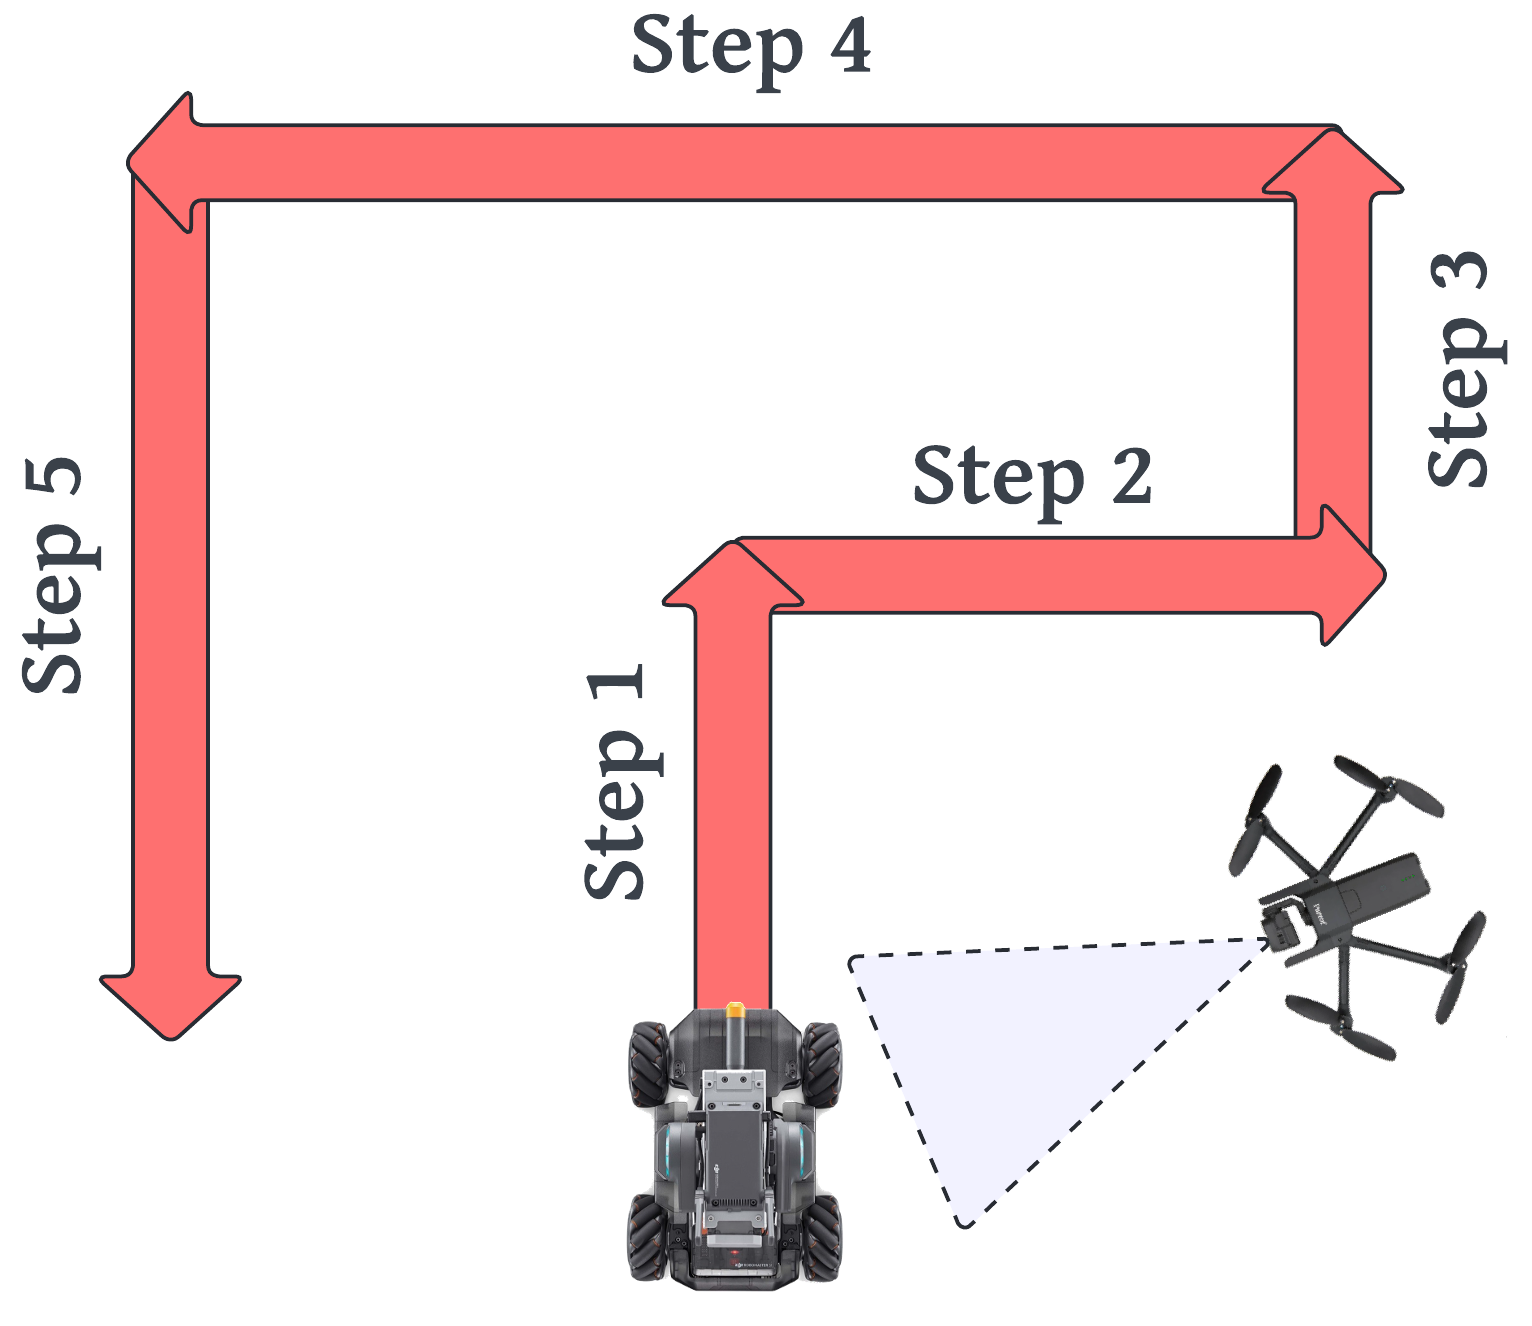
\includegraphics[width=0.8\linewidth]{chapter6/FIGS/fig-tracking-onepath.png}\\
{(a) Detail for 5-Step Example}
\end{minipage}
\begin{minipage}{0.35\linewidth}
\centering
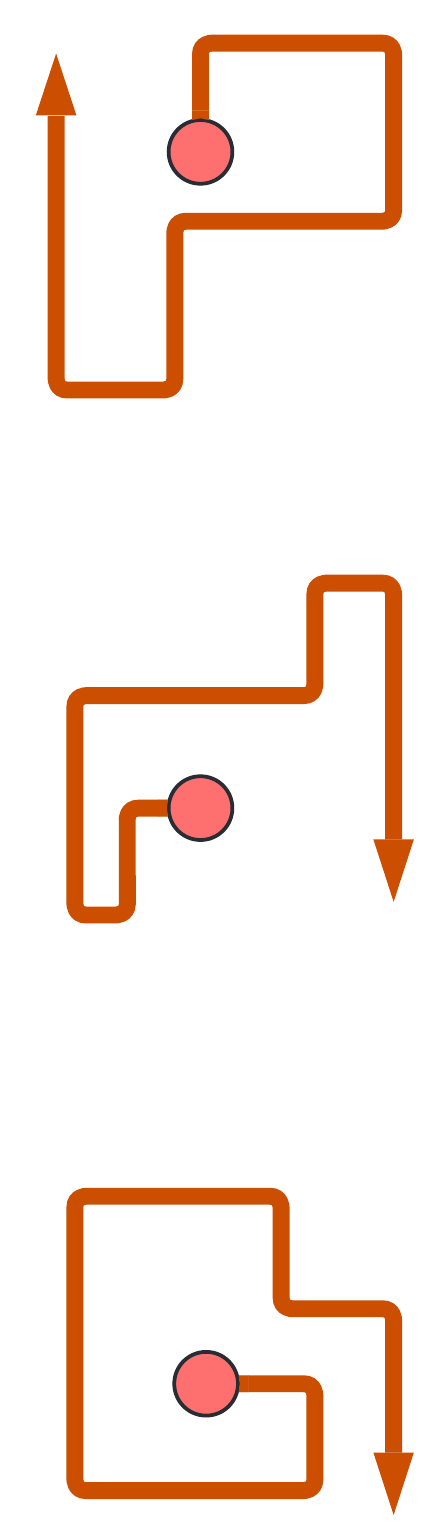
\includegraphics[width=0.35\linewidth]{chapter6/FIGS/fig-tracking-manypaths.png}\\
{(b) Other Examples}

\end{minipage}
\caption{Parameterized Random Walk}
\label{fig:tracking-path}
\end{figure}


To execute the benchmark, the target is placed in a large open outdoor
area.  The drone is manually piloted to the desired altitude, and its
FOV is adjusted to center the target. Once the drone has locked
onto its target, the target is instructed to start its pre-programmed
random walk and a timekeeper starts a stopwatch. The experiment
continues until one minute has elapsed or the drone loses the target
from its FOV.  The termination time and the black box footage of the
flight are logged for post-flight
scoring~(\S\ref{sec:tracking-scoring}).

\begin{figure}
\centering
\begin{minipage}{0.35\linewidth}
\centering
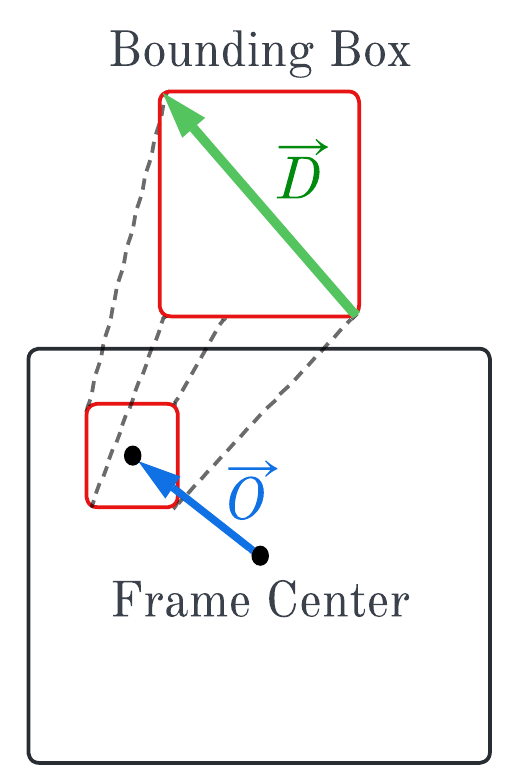
\includegraphics[width=\linewidth]{chapter6/FIGS/fig-tracking-scoring.png}
\caption{\small $\vec{O}$ \& $\vec{D}$}
\label{fig:o-d-calc}
\end{minipage}
\begin{minipage}{0.5\linewidth}
\small
\begin{equation}
	c_i = \norm{\vec{O}_i} / \norm{\vec{D}_i}\label{eq:2}
\end{equation}
\begin{equation}
	s_{i} = 1.1^{-c_i}\label{eq:3}
\end{equation}
\begin{equation}
	s_{\text{avg}} = \frac{\Sigma_i^n s_i}{n}\label{eq:4}
\end{equation}
\caption{Calculating Score\\[0.2cm]}
{\centering\small
$\norm{\vec{O}} = 0.11$, $\norm{\vec{D}} = 0.03$, $c = 3.67$ \\[0.1in]
$s_{10} = 1.1^{-c} = 0.70$ \\
$s_{20} = 1.2^{-c} = 0.51$ \\
$s_{30} = 1.3^{-c} = 0.38$ \\
}
\caption{Scoring Figure~\ref{fig:track-score-example}}
\label{fig:example-score-calcuclation}
\end{minipage}
\end{figure}

\begin{figure}
\centering
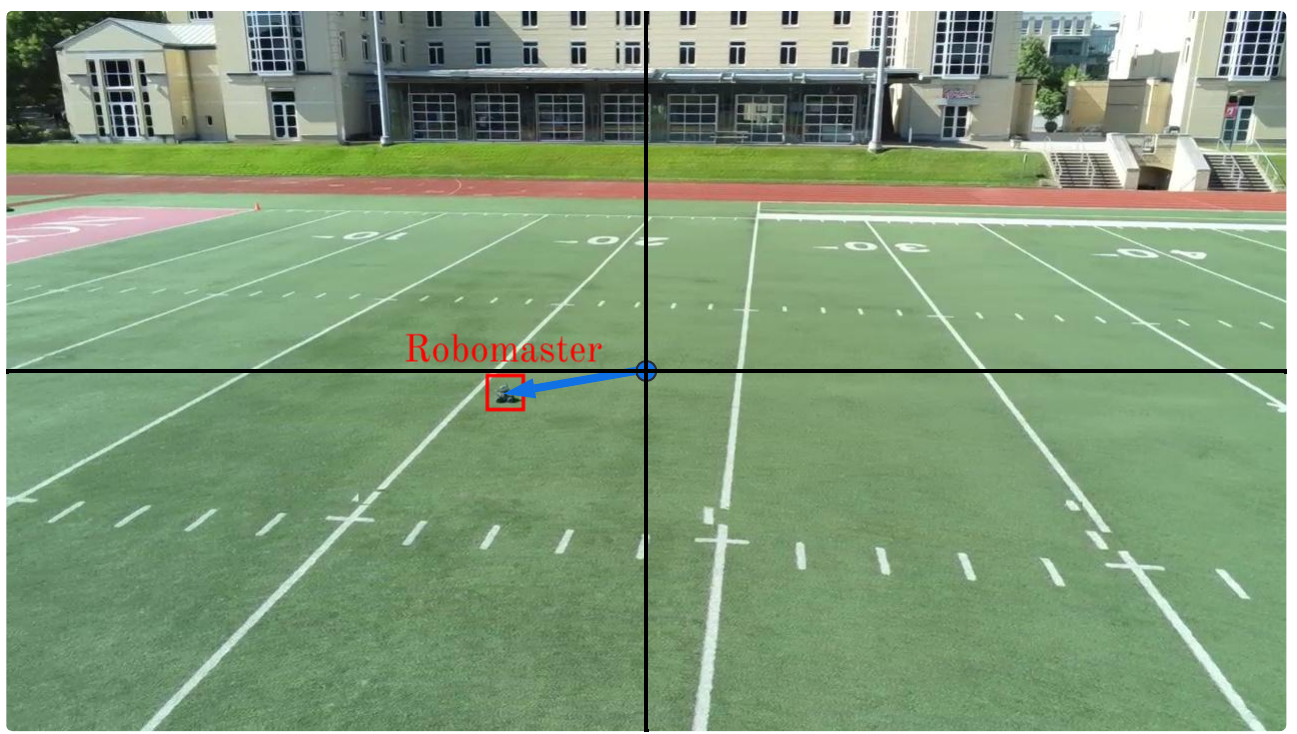
\includegraphics[width=0.9\linewidth]{chapter6/FIGS/fig-tracking-score-demo.png}
\caption{Example Frame for Scoring}
\label{fig:track-score-example}
\end{figure}

\subsection{Benchmark Scoring}
\label{sec:tracking-scoring}
In post-processing after a flight, I score the recorded video footage
using an automated process.  Figures~\ref{fig:o-d-calc} to
\ref{fig:example-score-calcuclation} show the scoring calculation,
using Figure~\ref{fig:track-score-example} as an example.  On each
frame, a DNN is first used to create a bounding box around the target.
With the center of the frame as the origin, the relative distance of
the target from the origin is obtained.  Using the notation shown in
Figure~\ref{fig:o-d-calc}, the pixel offset vector, $\vec{O}$, gives
the L2 distance of the target's centroid from the origin.  This is scaled
to the vector dimension, $\vec{D}$, of the bounding box to give the
centering ratio $c_i$~(formula \ref{eq:2}).  I then calculate the
score of the frame, $s_i$, by using an inverse exponential, as shown
in formula~\ref{eq:3}.  The rationale for using an exponential is to
super-linearly penalize distance from origin.  I use a compounding
10\% penalty in reporting my results, leading to the value of 1.1 in
formula~\ref{eq:3}.  Using $s_n$ to denote a penalty of n\%,
Figure~\ref{fig:example-score-calcuclation} shows the scores for
penalties of 10\%, 20\% and 30\% for the example frame in
Figure~\ref{fig:track-score-example}.  A score of zero is awarded when
the frame does not contain the target at all, or if the target is too
small to be detected in post-processing by a specified model.  In my
case, this model is YOLOv5x trained on aerial images of the target.

From the per-frame scores, the entire flight is scored by simple
averaging ~(formula \ref{eq:4}). The overall score, $s_{\text{avg}}$,
lies between $0$ and $1$, with higher being better. For
example, an average score of $0.70$ based on $s_{10}$ is achieved when
the drone is able to keep the target within about three normalized
lengths of the center of the FOV for the entire duration of the
flight.

\begin{table}
\centering
\begin{tabular}{|l|c|c|c|}
\hline
\textbf{Model} & \textbf{Latency} & \textbf{Throughput} & \textbf{mAP} \\
 & (ms) & (fps) & \\
\hline
YOLOv5s  & 28 & 25 & 56.8\\
YOLOv5m  & 37 & 20 & 64.1\\
YOLOv5l  & 42 & 20 & 67.3\\
\hline
\end{tabular}
\begin{captext}
  \\[0.1cm] \small The inference and throughput were obtained on the
  cloudlet~(\S\ref{sec:cloudlet}).  The mean average precision~(mAP)
  is from the YOLO documentation~\cite{Yolo}.
\end{captext}
\caption{YOLOv5 Performance in the SteelEagle Pipeline}
\label{fig:yolo-model-stats}
\end{table}


\subsection{Tracking Algorithm}
\label{sec:tracking-algorithm}
For this benchmark, I use the tracking algorithm used described in Section~\ref{sec:tracking-algorithm-advanced}. Figure~\ref{fig:yolo-model-stats} shows the latency, throughput and
accuracy of the three DNN models that are used for tracking in my
system, each trained on the Robomaster target.  Even using the slowest of these as Stage-2 of
Orient+Decide$_d$ only adds 42 milliseconds of latency to the base
value of 527~ms~(Figure~\ref{fig:ooda-scaling}).  Its throughput of
20~fps is well above that of the bottleneck~(Act$_{fg}$).  However,
there may be situations where load on a multi-tenant cloudlet may need
to be reduced, and the smaller models may be valuable for that
purpose.

\section{Visual Object Tracking: Results}
\label{sec:tracking-results}
The basic question I ask about tracking is as follows:
\begin{itemize}
\item{\em How well does my platform follow a target that makes random,
  rapid changes in direction?}
\end{itemize}
As Figure~\ref{fig:tracking-best} shows, my platform is able to track
the target on my benchmark even at the fastest speed~(3.5~m/s)
without ever completely losing it.  However, as the scores show, the
target is off-center in some frames at all speeds.  As target speed
decreases, the score achieved shows a modest improvement.  The results
shown here are based on the best model for each speed.  This
dependence is explored further in \S\ref{sec:tracking-models}.

\begin{figure}
\centering
\begin{minipage}{0.49\linewidth}
\centering
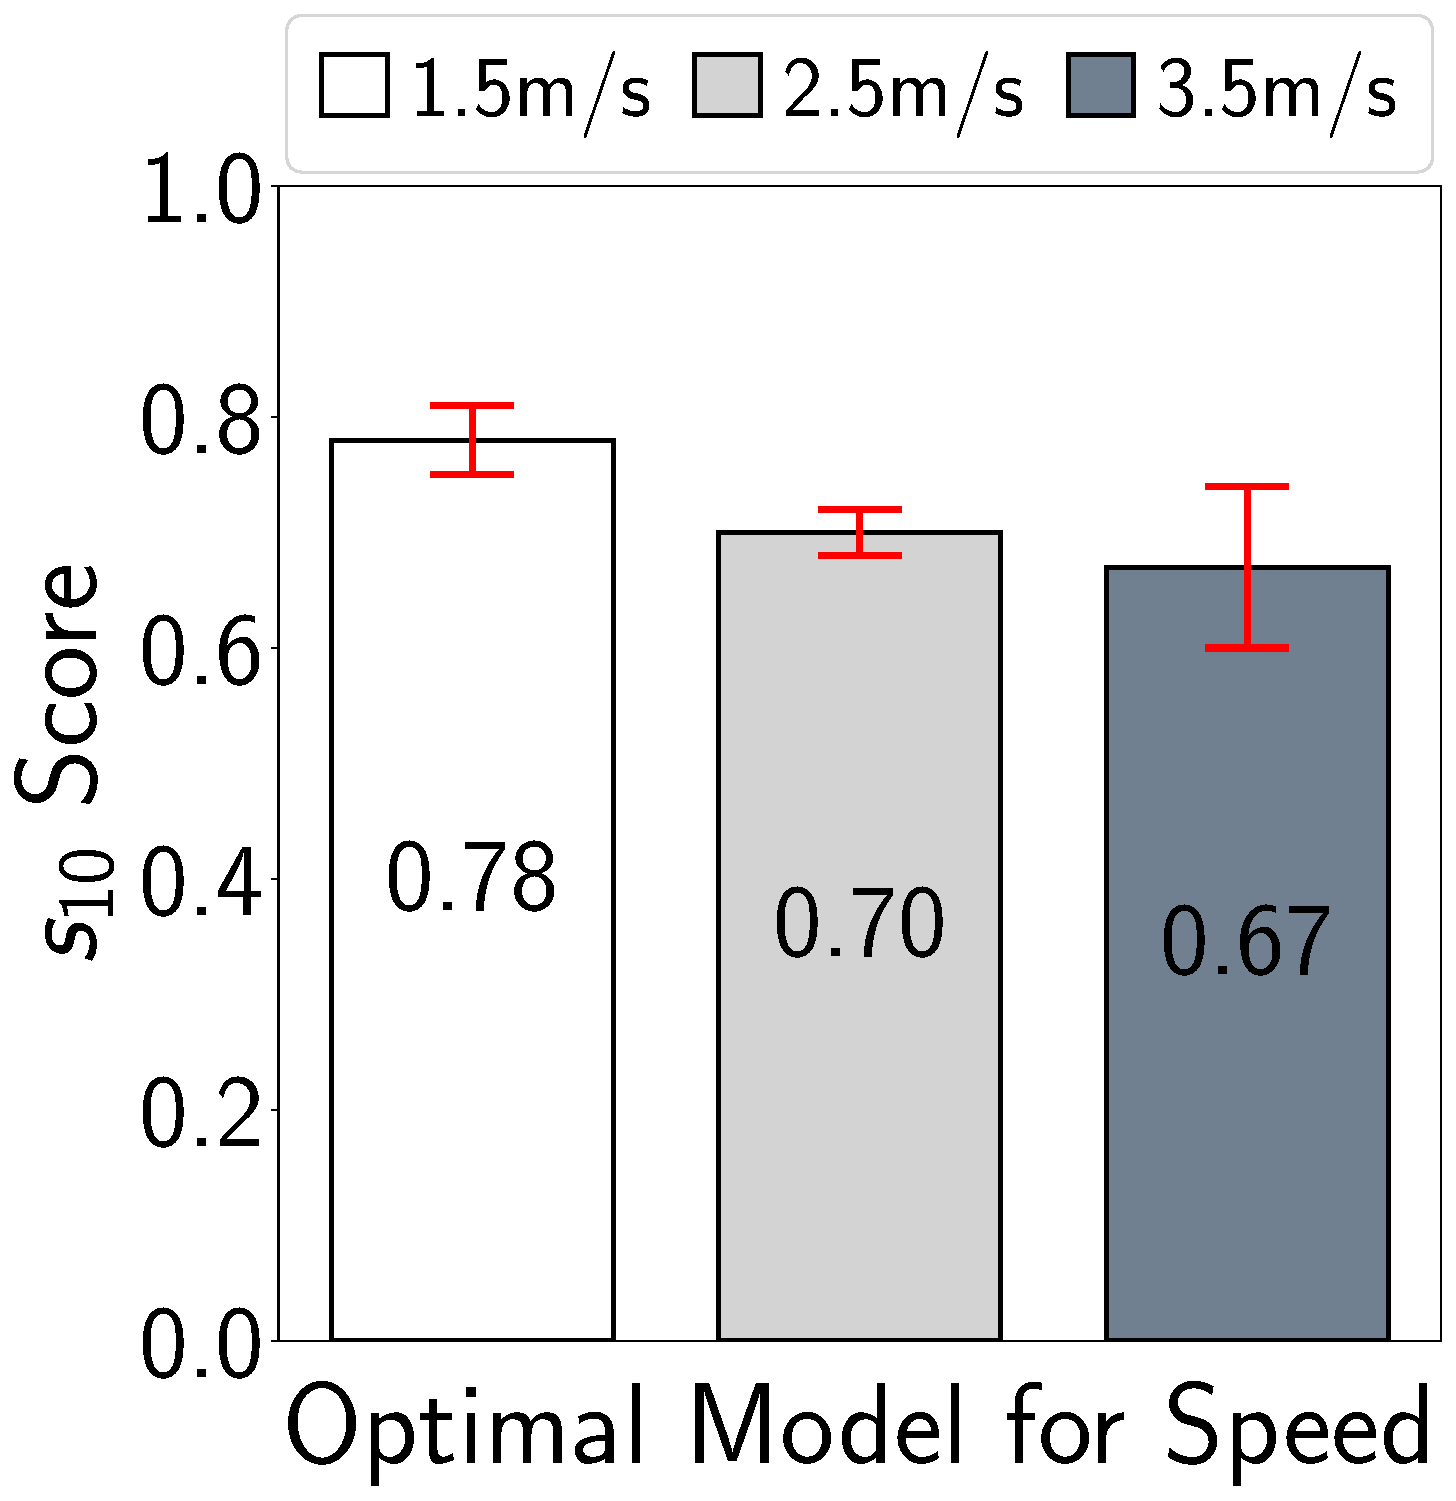
\includegraphics[width=1.0\linewidth]{chapter6/FIGS/fig-tracking-best.pdf}\\
\caption{Baseline Scores}
\label{fig:tracking-best}
\end{minipage}
\begin{minipage}{0.49\linewidth}
\centering
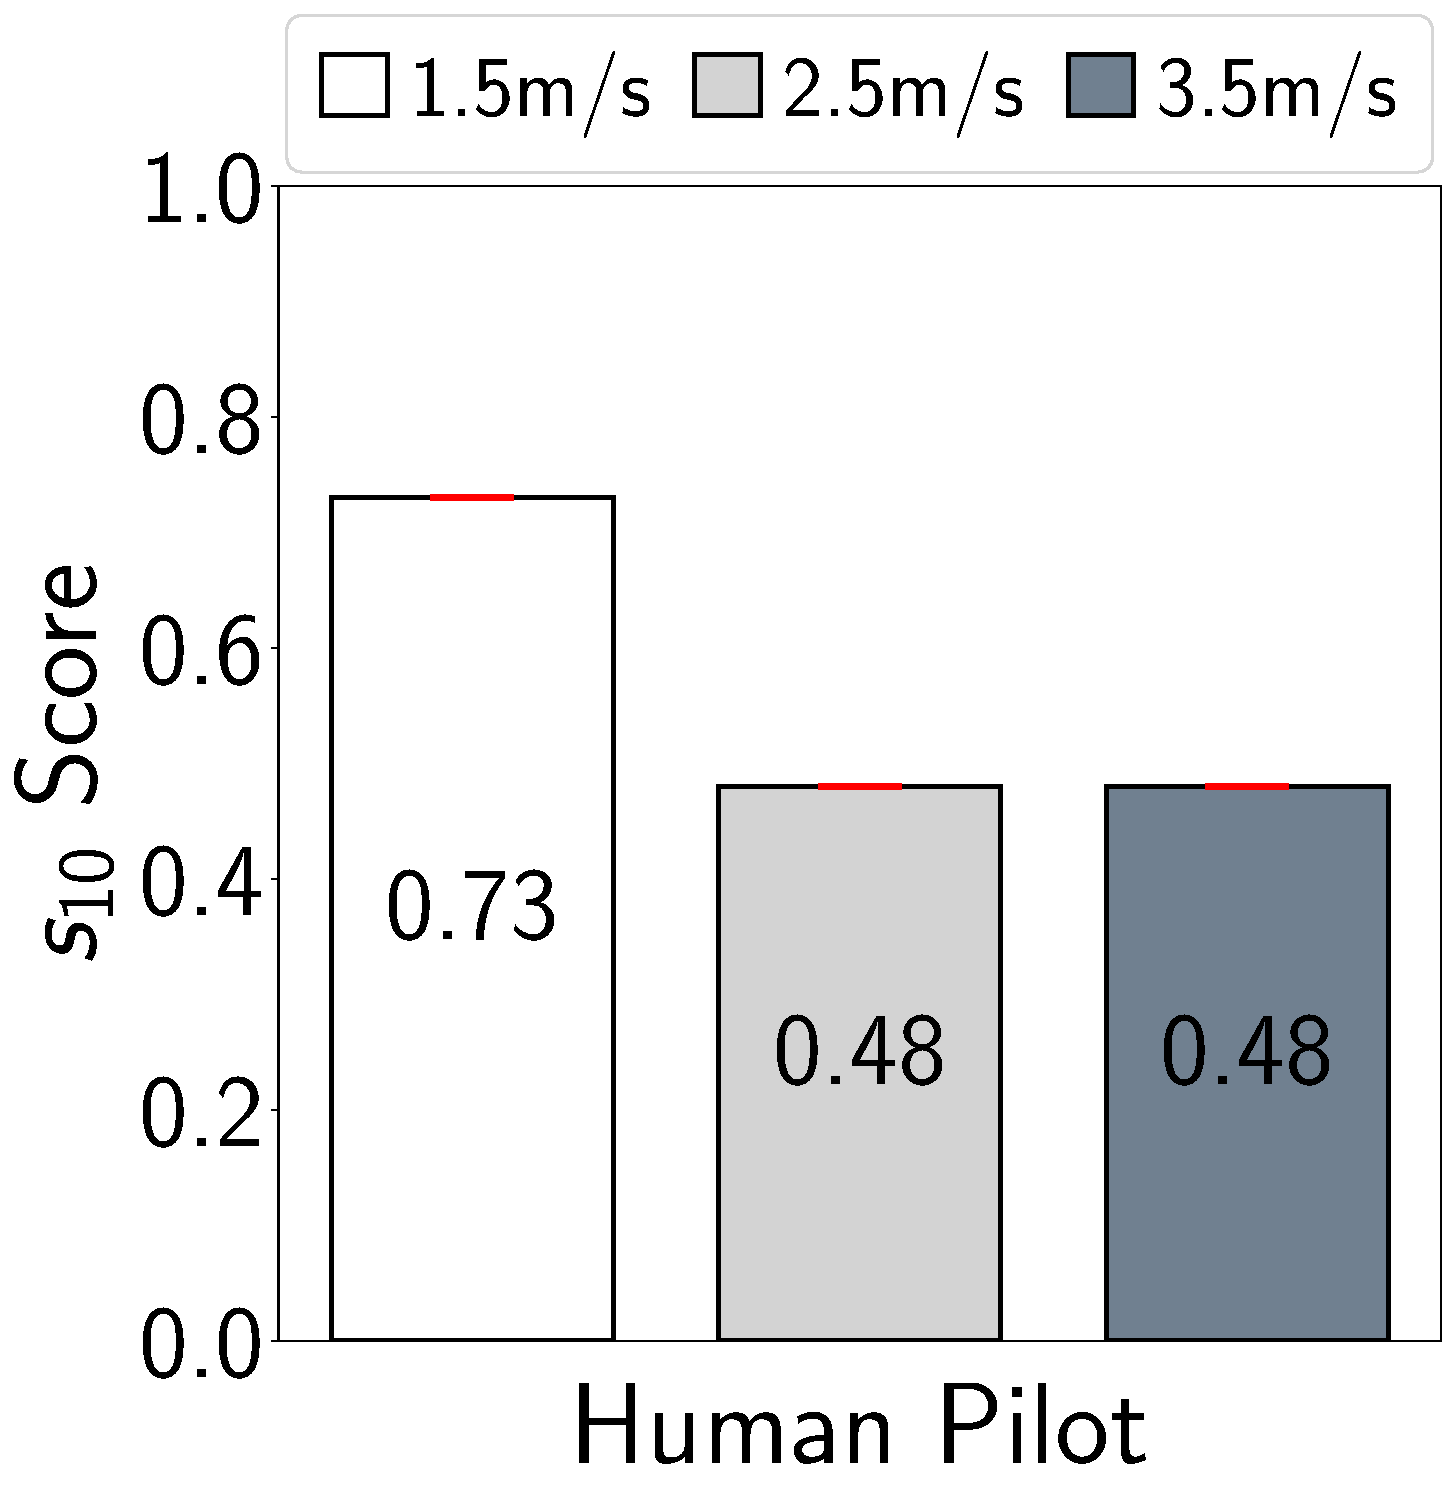
\includegraphics[width=1.0\linewidth]{chapter6/FIGS/fig-tracking-human.pdf}\\
\caption{Human Pilot}
\label{fig:tracking-human}
\end{minipage}
\end{figure}

As in the case of obstacle avoidance, I ask how well an experienced
human pilot performs under identical conditions. The pilot is held
constant from \S\ref{sec:avoidance}.
Figure~\ref{fig:tracking-human} shows how well the human pilot scored
on the benchmark.  Comparing Figures~\ref{fig:tracking-best} and
~\ref{fig:tracking-human}, I see that the autonomous drone and the
human are comparable at 1.5~m/s, but at higher speeds the autonomous
drone outperforms the human.  This is in contrast to obstacle
avoidance~(Figures~\ref{fig:avoid-best} and \ref{fig:avoid-human}),
where the human consistently outperformed the autonomous drone.  I
conjecture that at least part of this difference is attributable to
the fact that the obstacle course is static, and hence subconscious
pre-planning by the human helps in navigating it.  In contrast, the
human is no better than the drone in anticipating random turns made by
the target.  At higher speeds, raw reaction speed~(i.e., the
\ooda~loop) is all that matters, and the autonomous drone proves to be
better in this regard.

\begin{figure}
\centering
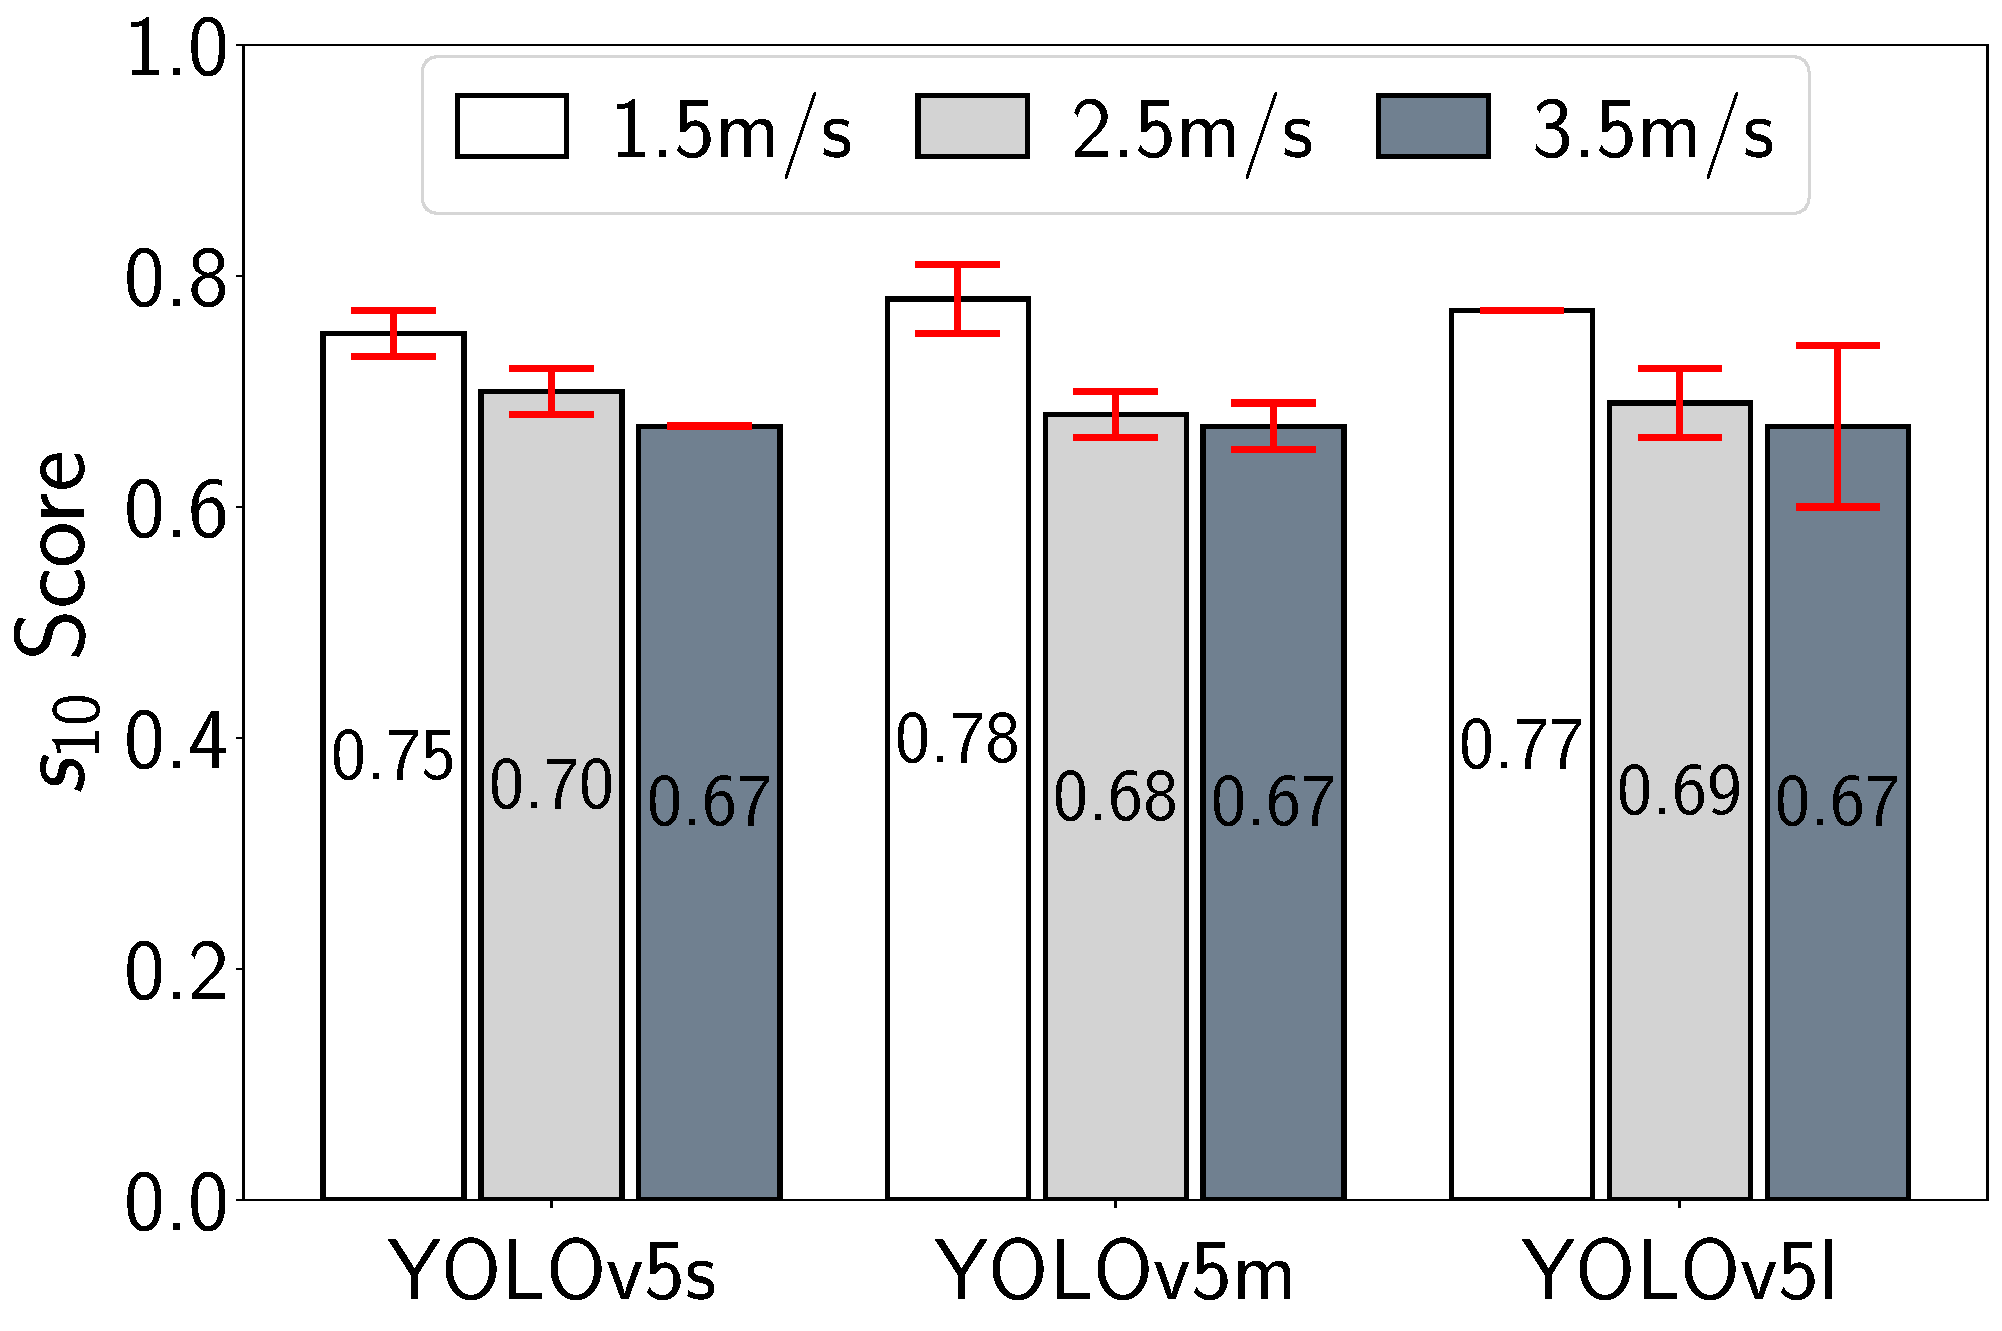
\includegraphics[width=0.8\linewidth]{chapter6/FIGS/fig-tracking-models.pdf}
\caption{\small Impact of YOLO Model on Tracking Benchmark}
\label{fig:track_models}
\end{figure}

\subsection{Impact of Model Accuracy}
\label{sec:tracking-models}

Since multiple DNN models are available to use in
tracking~(Figure~\ref{fig:yolo-model-stats}), I ask the following
question:
\begin{itemize}
\item{\em Does the use of a better model improve tracking?}
\end{itemize}
Figure~\ref{fig:track_models} presents my results.  For any given
speed, there is little difference across models.  The increased
cloudlet load of a more accurate model does not pay off.  However, it
should be noted that this observation may only be true for this
specific tracking benchmark.  As described
in~\S\ref{sec:tracking-description}, the benchmark is defined as being
conducted in an open area free of clutter.  If I were to create a
different tracking benchmark that embodies extensive clutter~(such as
that of a busy street filled with moving cars, bicycles, and
pedestrians, along with static objects such as parked cars and trees),
the results may be quite different. In that case, the improved
accuracy of the larger models may prove decisive. The creation of such a benchmark could be a subject of future work.

\begin{figure}
\centering\small
\begin{minipage}{0.8\linewidth}
\centering
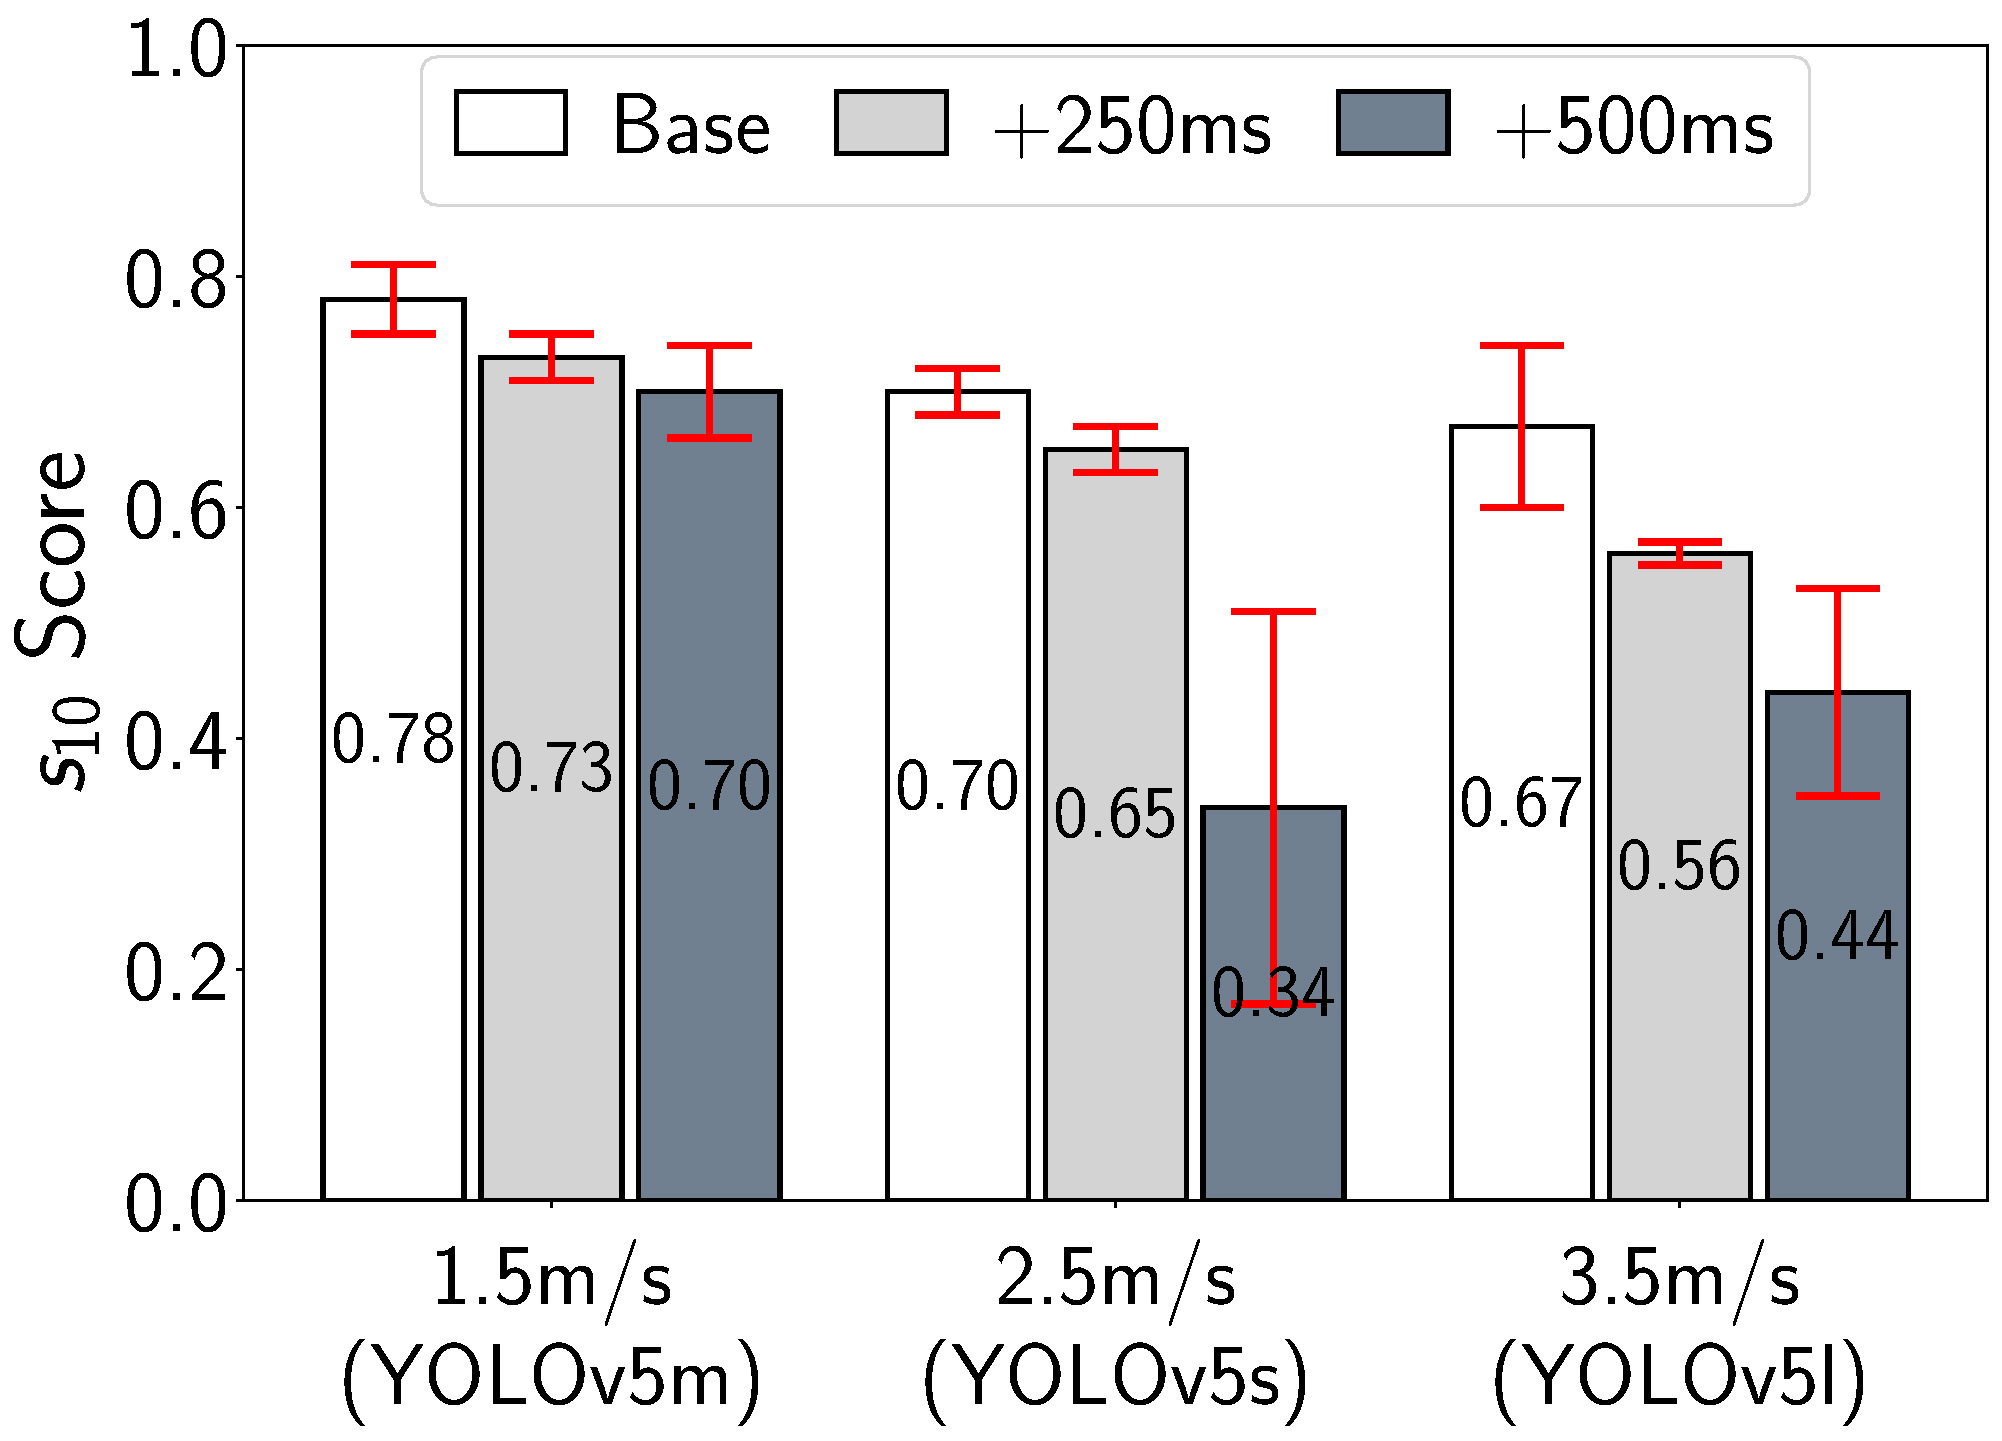
\includegraphics[width=0.98\linewidth]{chapter6/FIGS/fig-tracking-latency.pdf}\\
(a) Additional Latency
\end{minipage}
\begin{minipage}{0.8\linewidth}
\centering
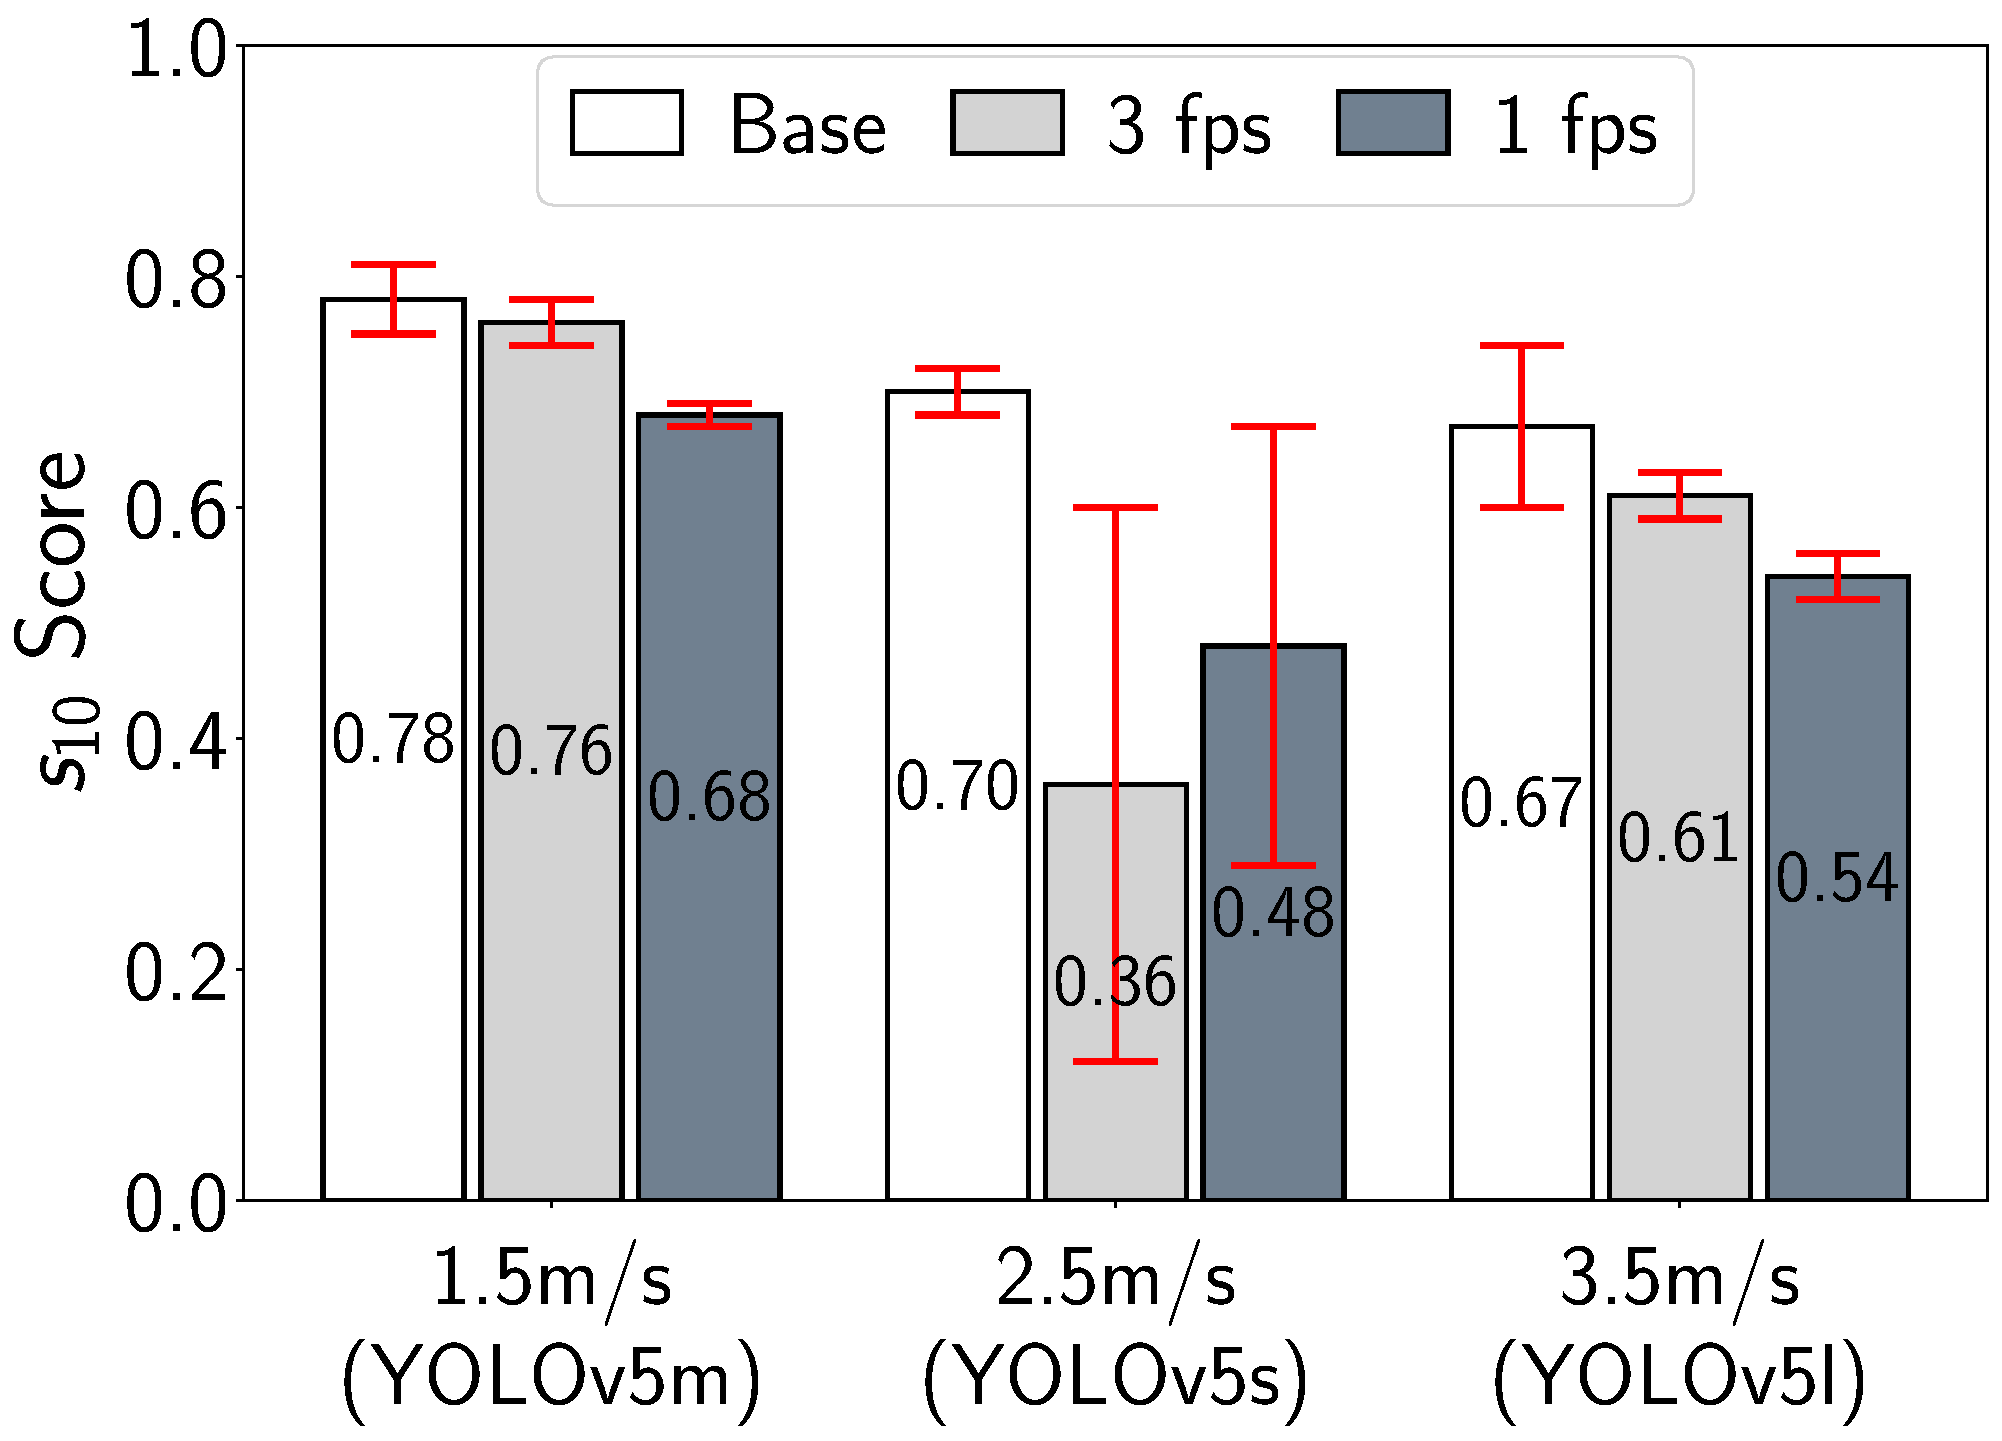
\includegraphics[width=0.98\linewidth]{chapter6/FIGS/fig-tracking-fps.pdf}\\
(b) Reduced Throughput
\end{minipage}
\caption{Impact of Latency and Throughput on Tracking}
\label{fig:tracking-latency-throughput}
\end{figure}

\subsection{Impact of Latency \& Throughput}
\label{sec:tracking-factors}

As in the case of obstacle avoidance~(\S\ref{sec:avoidance-factors}),
I ask:
\begin{itemize}
\item{\em What is the impact of latency or throughput degradation of
    the \ooda~loop on benchmark score?}
\end{itemize}
Figure~\ref{fig:tracking-latency-throughput}(a) shows what happens
when additional latency of 250~ms and 500~ms are added to the
\ooda~loop.  For all target speeds and models, there is a noticeable
drop in benchmark score.  The drop is worse at higher speeds.  This is
directly attributable to the inability of the more sluggish \ooda~loop
to keep the target centered in the FOV.  At higher speeds, the drone
often loses sight of the target early in the tracking.  This results
in a zero score for the remaining frames of that experiment, and hence
an overall low average score.

Figure~\ref{fig:tracking-latency-throughput}(b) shows the same trend
when \ooda~loop throughput is artificially throttled to 3~fps or
1~fps.  At all target speeds and for all models, there is a noticeable
drop in benchmark score.  This drop is greater at higher speeds.

The results in Figures~\ref{fig:tracking-latency-throughput}(a) and
(b) confirm that both end-to-end latency and bottleneck throughput are
important independent factors in determining tracking ability.
Optimizing one at the cost of the other, as occurs when using
strategies such as batching of operations, is unlikely to be
beneficial.


\section{Obstacle Avoidance: Benchmark}
\label{sec:avoidance}
Obstacle avoidance is vital for drone flights at low altitude (up to a
few hundred feet) in urban or forested settings. Otherwise, being restricted to only high altitude flight impairs visual detections and hides many details.  The most dangerous obstacles are
typically trees, lightposts, and telephone poles, which can easily
reach altitudes usually used by drones. Being  relatively thin,
they are difficult to detect from afar.  

Efficient avoidance of such obstacles is a challenge.  Since drone
flight is limited by battery life (typically on the order of 30-50
minutes), bypassing obstacles without wasting too much flight time is
important. If flight is too slow or avoidance maneuvers are too
convoluted, mission performance will be impaired.  At the same time,
reckless flight could be catastrophic.  Striking the right balance
between safety and speed for the given flight conditions is essential.
Since effective but rapid avoidance of obstacles is a valuable
capability in a drone, this task is a good candidate for an agility
benchmark.

\subsection{Benchmark Requirements}
\label{sec:avoidance-requirements}

A good benchmark for this task should capture the essential difficulty
of obstacle avoidance.  It should be parameterized, so that it is easy to
vary the difficulty of the benchmark.  The benchmark should only use
standardized, off-the-shelf components that can be easily purchased or
fabricated.  There should be no ambiguity in the experimental setup or
interpretation of results, thereby simplifying independent attempts to
reproduce published experimental results.
\S\ref{sec:avoidance-description} presents my candidate benchmark
that meets these requirements.

\subsection{Benchmark Description}
\label{sec:avoidance-description}

\begin{figure}
    \centering
    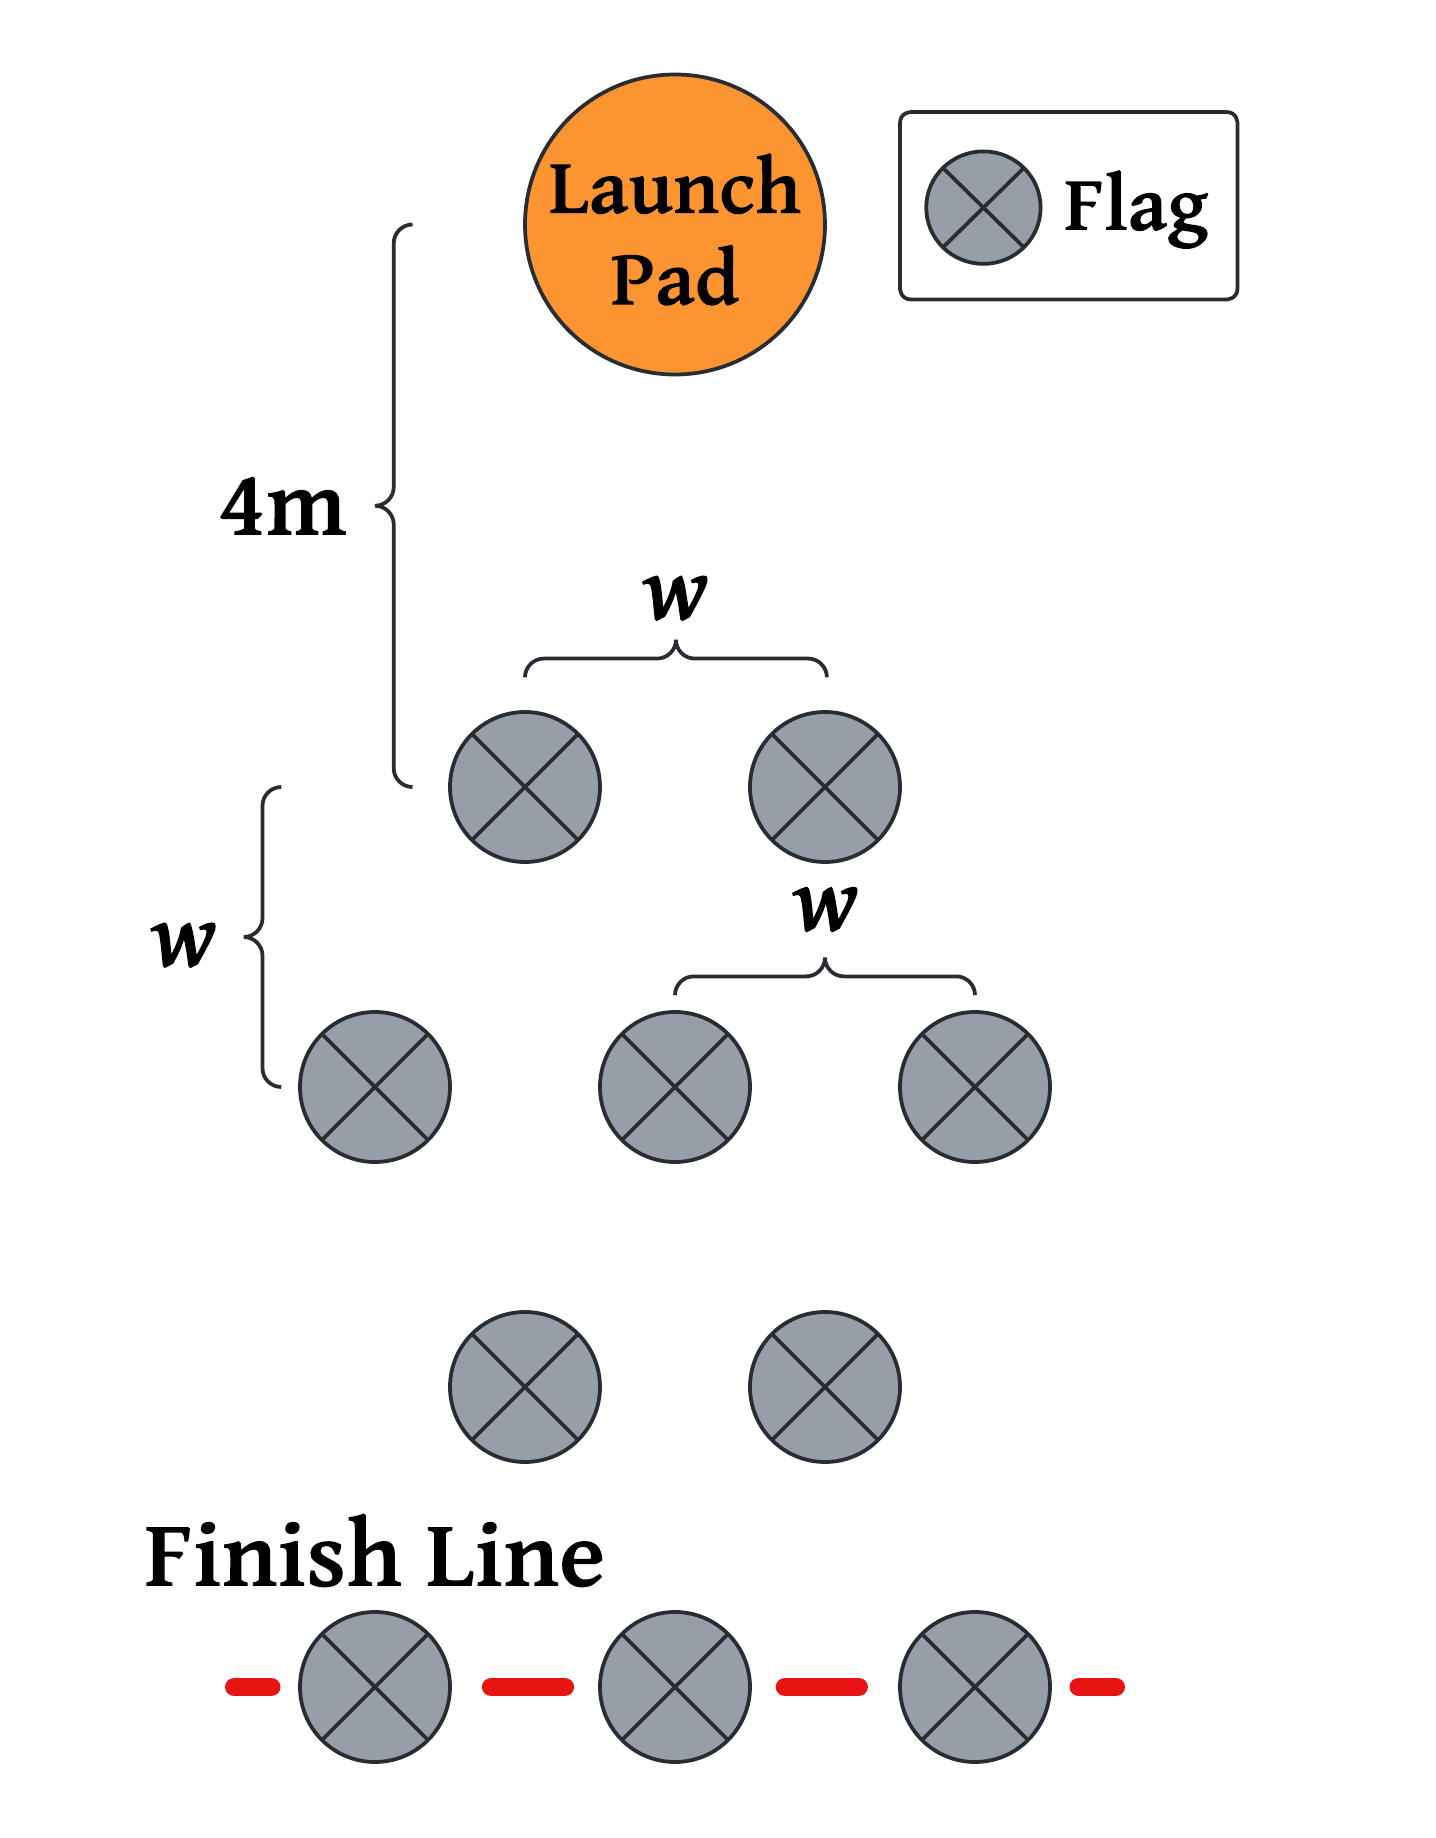
\includegraphics[trim=-4cm 0 0 0, width=0.5\linewidth]{chapter6/FIGS/fig-obstacle-course.png}
    \caption{Obstacle Course Layout}
    \label{fig:obstacle-course}
\end{figure}

To emulate tall and skinny obstacles such as lightposts, I use 1.8~m
long drone racing flags.  The flags are
arranged in a precisely-defined slalom
pattern~(Figure~\ref{fig:obstacle-course}), that forces a drone to
sequentially evade several obstacles.  The difficulty of the course is
controlled by a spacing parameter, $w$, that determines the separation
of the flags along both the azimuth and range axes.  A smaller value
of $w$ defines a more difficult course because of higher density of
obstacles in both directions.  All my experiments were conducted with
4 tiers of obstacles.  Adding more tiers to make the obstacle course
longer, while preserving obstacle spacing, would add further
difficulty to the course.  The drone's goal is to navigate the course
as fast as possible, without touching the flags or striking a
flagpole.  The metric of interest is the transit time through the
course.

To execute this benchmark, the obstacle course is set up as in
Figure~\ref{fig:obstacle-course}.  The drone is placed on a pad that
is centered 4~m in front of the leading line of flags.  A human
spotter stands a safe distance behind the drone, and a human
timekeeper is positioned along the finish line.  The remote
pilot-in-command (RPIC) continuously monitors the video stream from
the drone, and stands ready to wrest back manual control if the
drone's autonomous flight software appears to be getting it into
trouble.  Such a manually aborted flight is scored as ``Did Not
Finish~(DNF).''  A flight in which the drone touches a flag
or pole is also scored as DNF.

The drone takes off and then hovers at an altitude of 1~m.  It
is then directed to autonomously move to a destination beyond the
obstacle course. When forward motion begins, the spotter visually
signals the timekeeper to start a stopwatch. The spotter then follows
the drone through the course, warning the RPIC of imminent collision,
if any.  Such a warning aborts the experiment without damage to the
drone.  On a successful flight, timing is stopped as soon as the
trailing end of the drone crosses the finish line.  We deem an
obstacle spacing, $w,$ as viable if the drone successfully flies
through the course on at least 80\% of its attempts.  The average time
of these successful flights at the smallest viable $w$ is the figure
of merit. For small values of $w$, a more agile drone can fly more
aggressively and therefore requires less time to complete the benchmark.
However, at higher values of $w$, agility may not be important because
the obstacle course easier.

\begin{table}
\small
	\centering
        \begin{tabular}{|c|c|c|}
		\hline
		\textbf{Model} & \textbf{Latency (ms)} & \textbf{Throughput (fps)} \\
		\hline
		MiDaS Small & 61 & 10 \\
		DPT Hybrid & 105 & 8 \\
		DPT Large & 132 & 7 \\
		\hline
	\end{tabular}
\begin{captext}
\centering
    \\[0.1cm]
  \small These numbers were obtained on the cloudlet described in
  \S\ref{sec:cloudlet}
\end{captext}
\caption{Inference Speeds of MiDaS DNN Models}
\label{tab:midas-model-stats}
\end{table}

\subsection{Benchmark Scoring}
\label{sec:avoidance-scoring}

The average time, $t_{\text{avg}}$, for multiple experimental runs at
the lowest viable $w$ is a raw measure of agility.  However, this needs
to be normalized with respect to attributes other than agility.
For example, a drone whose top speed is low relative to other drones
may be penalized unfairly when measuring agility.  A low value of
$t_{\text{avg}}$ in that case is not due to a poor \ooda~loop, but
simply reflects the ``brute force'' attribute of top speed.  The
normalization is performed by removing flags from the course and
conducting a control experiment at top speed.  We denote the average
time for multiple runs of the control experiment as $t_{\text{min}}$.
The score, $S_w$, is then given by:
\begin{equation}
	S_w = \frac{t_{\text{min}}}{t_{\text{avg}}}\label{eq:1}
\end{equation}
Scores for this benchmark thus lie in the interval $0 < S_w \leq 1$
where $S_w = 1$ is the best possible score. A score of 0 is awarded
when a drone cannot achieve a successful completion rate of at least
80\% of the runs for the given value of $w$.

\subsection{Depth Sensing}
\label{sec:midas}

I use the same MiDaS-based avoidance algorithm described in Section~\ref{sec:midas-algorithm}. For this task, the \ooda~loop determines the speed and accuracy with which the drone can acquire fresh frames, execute the MiDaS algorithm on them, calculate new headings for safety, and perform actuations towards those headings.  In the context of \S\ref{sec:cloudlet}, MiDaS represents Stage-2 of cloudlet processing.  Stage-3 is the processing of MiDaS output to determine a new heading, and generating the actuation command. Figure~\ref{fig:midas-sample-course} shows the algorithm running on a setup benchmark course.

\begin{figure}
	\begin{minipage}{0.495\linewidth}
		\centering
		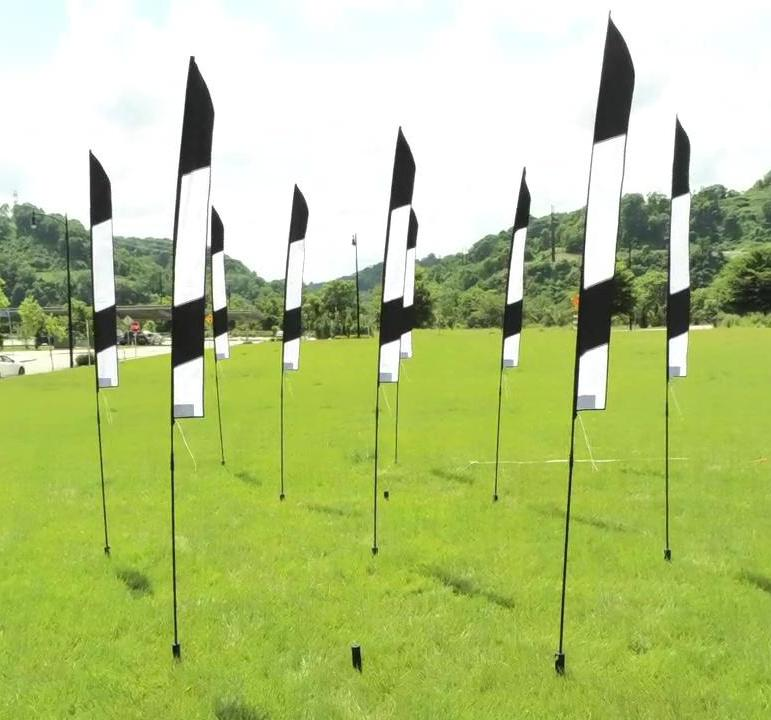
\includegraphics[width=0.8\linewidth]{chapter6/FIGS/fig-obstacle-course-drone-pov.jpg}\\
		{(a) Raw Input}\\
	\end{minipage}
	\begin{minipage}{0.495\linewidth}
		\centering
		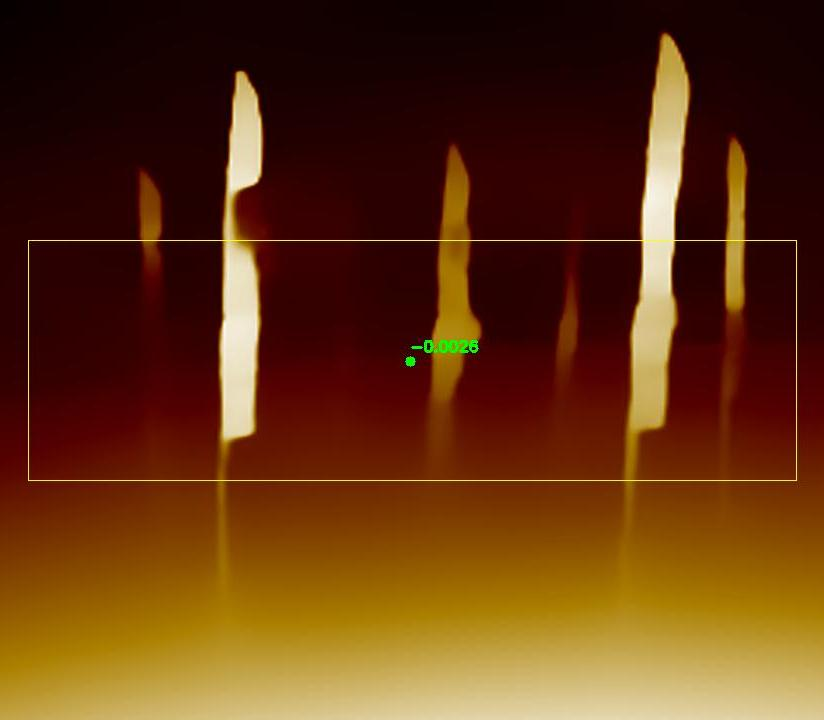
\includegraphics[width=0.8\linewidth]{chapter6/FIGS/fig-obstacle-course-midas.jpg}\\
		{(b) Output of MiDaS}\\
	\end{minipage}
\caption{MiDaS Running on the Benchmark Course}
\label{fig:midas-sample-course}
\end{figure}

I explore three DNN variants of MiDaS that vary in accuracy and speed:
{\em MiDaS Small,} {\em DPT Hybrid}, and {\em DPT Large}.  MiDaS Small
prioritizes throughput and inference latency at the cost of lower
accuracy. DPT Hybrid strikes a compromise between speed and accuracy.
DPT Large prioritizes accuracy above all else.  Figure
\ref{tab:midas-model-stats} shows the inference latency and throughput
of these three models on my cloudlet.  I explore the use of all three in my experiments.


\section{Obstacle Avoidance: Results}
\label{sec:avoidance-results}
The most basic questions in my evaluation are as follows:
\begin{itemize}
\item{\em What is the smallest value of $w$ for which the drone can
    successfully complete the benchmark?}

\item{\em At that $w$, how fast is benchmark completion?}

\item{\em As $w$ is increased, how much faster is the drone able to
    complete the benchmark?}
\end{itemize}

Initial experiments showed that 2~m is the smallest value of $w$
that meets my criterion for successful benchmark completion (i.e., at
least 80\% of the flights are successful).  Using the scoring
criterion described in \S\ref{sec:avoidance-scoring},
Figure~\ref{fig:avoid-best} shows how well the drone
 did for $w$ set
to 2~m, 2.5~m, and 3.0~m.  The results shown are the mean of 5 runs of
each experiment.  For each value of $w$, the drone results were
obtained with the choice of MiDaS model that gave the best results.
These choices were DPT Large for $w = $2~m, and MiDaS Small for $w =
2.5$~m and $w = 3$~m.  The scores of 0.13 to 0.2 show that the drone
suffers almost an order of magnitude slowdown when avoiding obstacles,
relative to its unimpeded traversal of the course.  This is the price
of having to execute the \ooda~loop shown in
Figure~\ref{fig:ooda-scaling}, with the additional Stage-2 and Stage-3
processing for depth estimation described in \S\ref{sec:midas}.  As
$w$ is increased from 2~m to 3~m, Figure~\ref{fig:avoid-best} shows
the score improving from 0.13 to 0.2.  This confirms my expectation
that less challenging courses are faster to traverse.

Since humans are the standard against which AI systems are measured,
I ask how a human pilot does under identical conditions. To
explore this, an experienced RPIC with several dozen hours of flight
time on the Parrot ANAFI platform manually executed the benchmark for
the same values of $w$. The \ooda~loop is now cyber-human: the RPIC uses the drone's live video stream to manually fly it.  Of course, a human also
has foreknowledge of the obstacle course and can subconsciously
leverage that knowledge in planning the drone's flight.  In contrast,
the autonomous drone is purely reactive --- what it sees right now is
all that it knows.

Figure~\ref{fig:avoid-human} presents my results.  Relative to
unimpeded traversal of the course, the scores of 0.76 to 0.46 show
that even the RPIC suffers a slowdown.  However, the slowdown is much
smaller than that suffered by the autonomous drone in
Figure~\ref{fig:avoid-best}.  Since the drone hardware and wireless
network are identical in the two sets of experiments, the difference
is due to the superior \ooda~loop of the human.  There is
clearly ample headroom for improvement of the drone's \ooda~loop.

\begin{figure}
\centering
\begin{minipage}{0.45\linewidth}
\centering
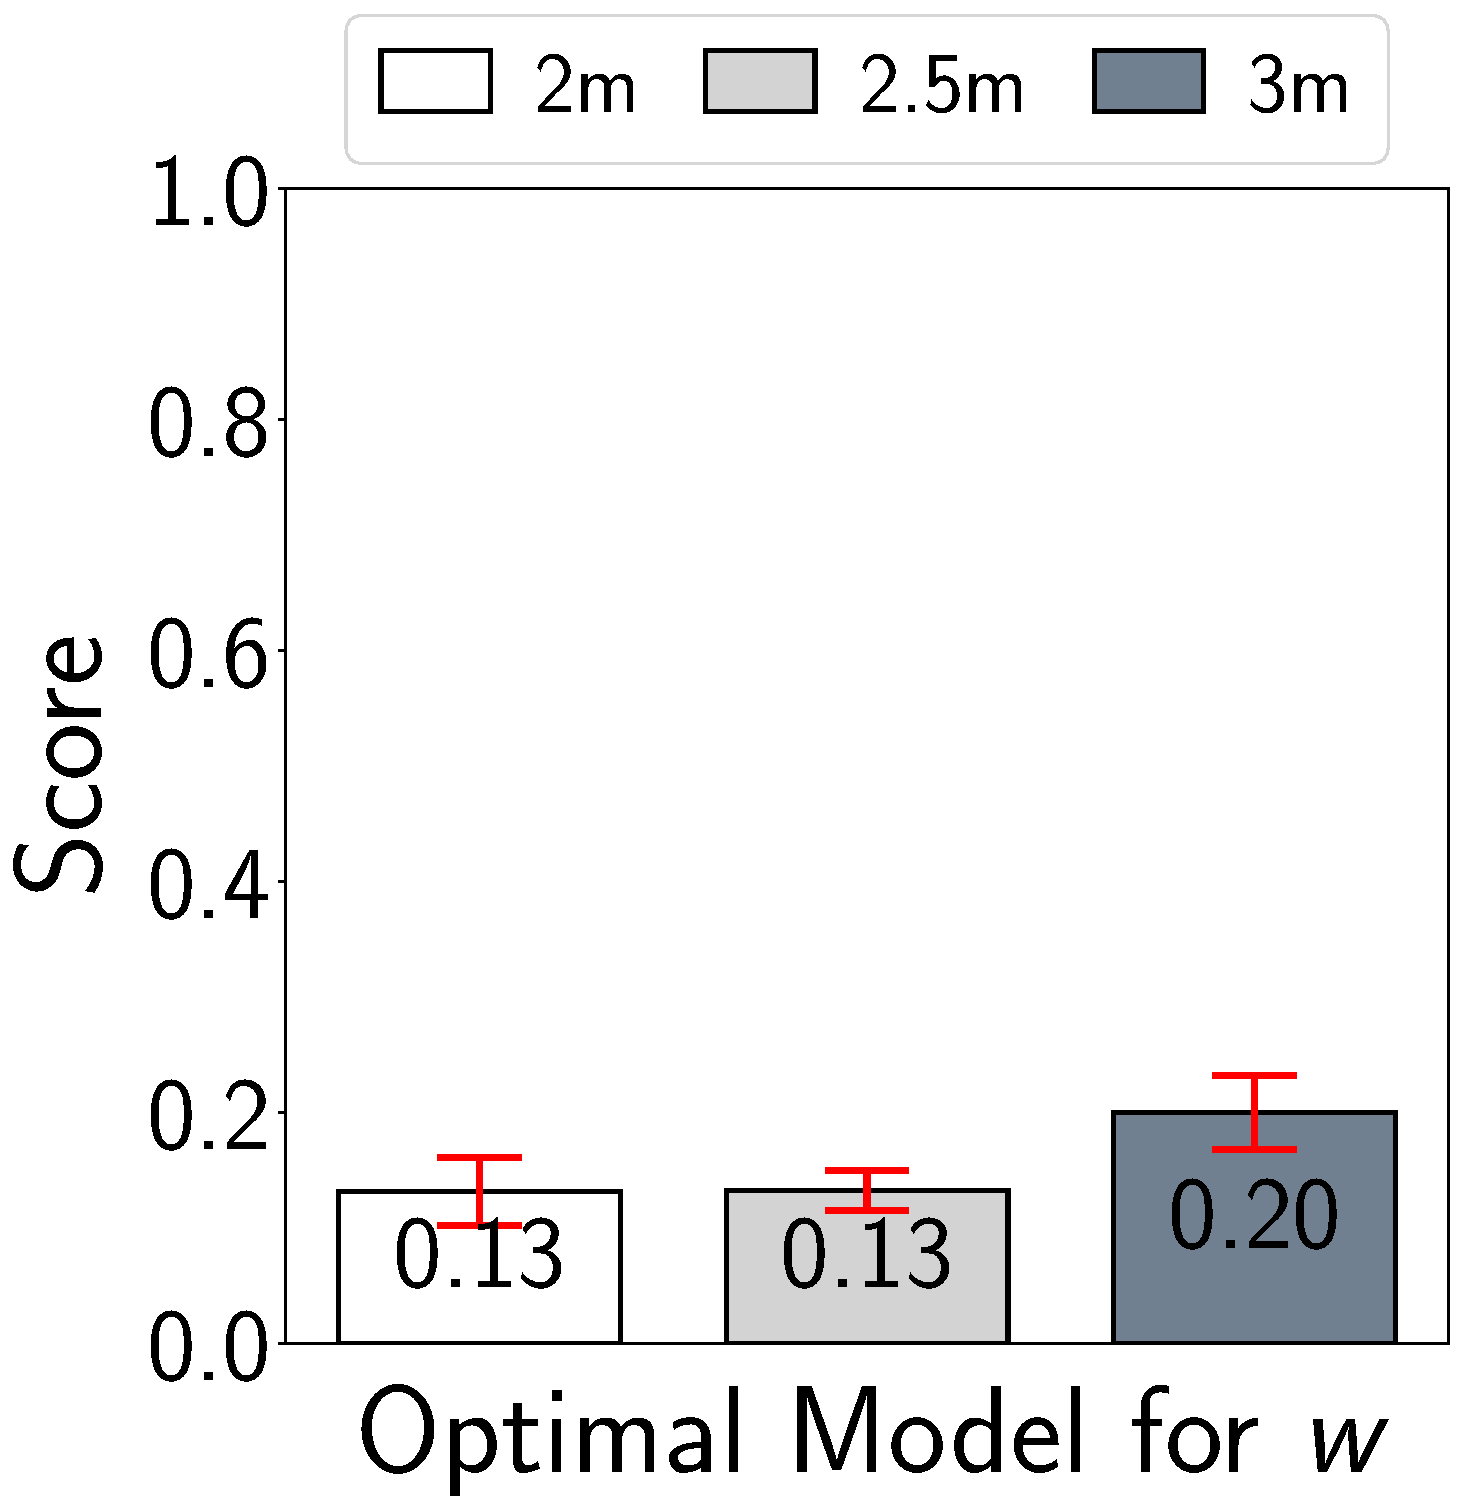
\includegraphics[width=1.0\linewidth]{chapter6/FIGS/fig-avoidance-best.pdf}\\
\caption{Baseline Scores}
\label{fig:avoid-best}
\end{minipage}
\begin{minipage}{0.45\linewidth}
\centering
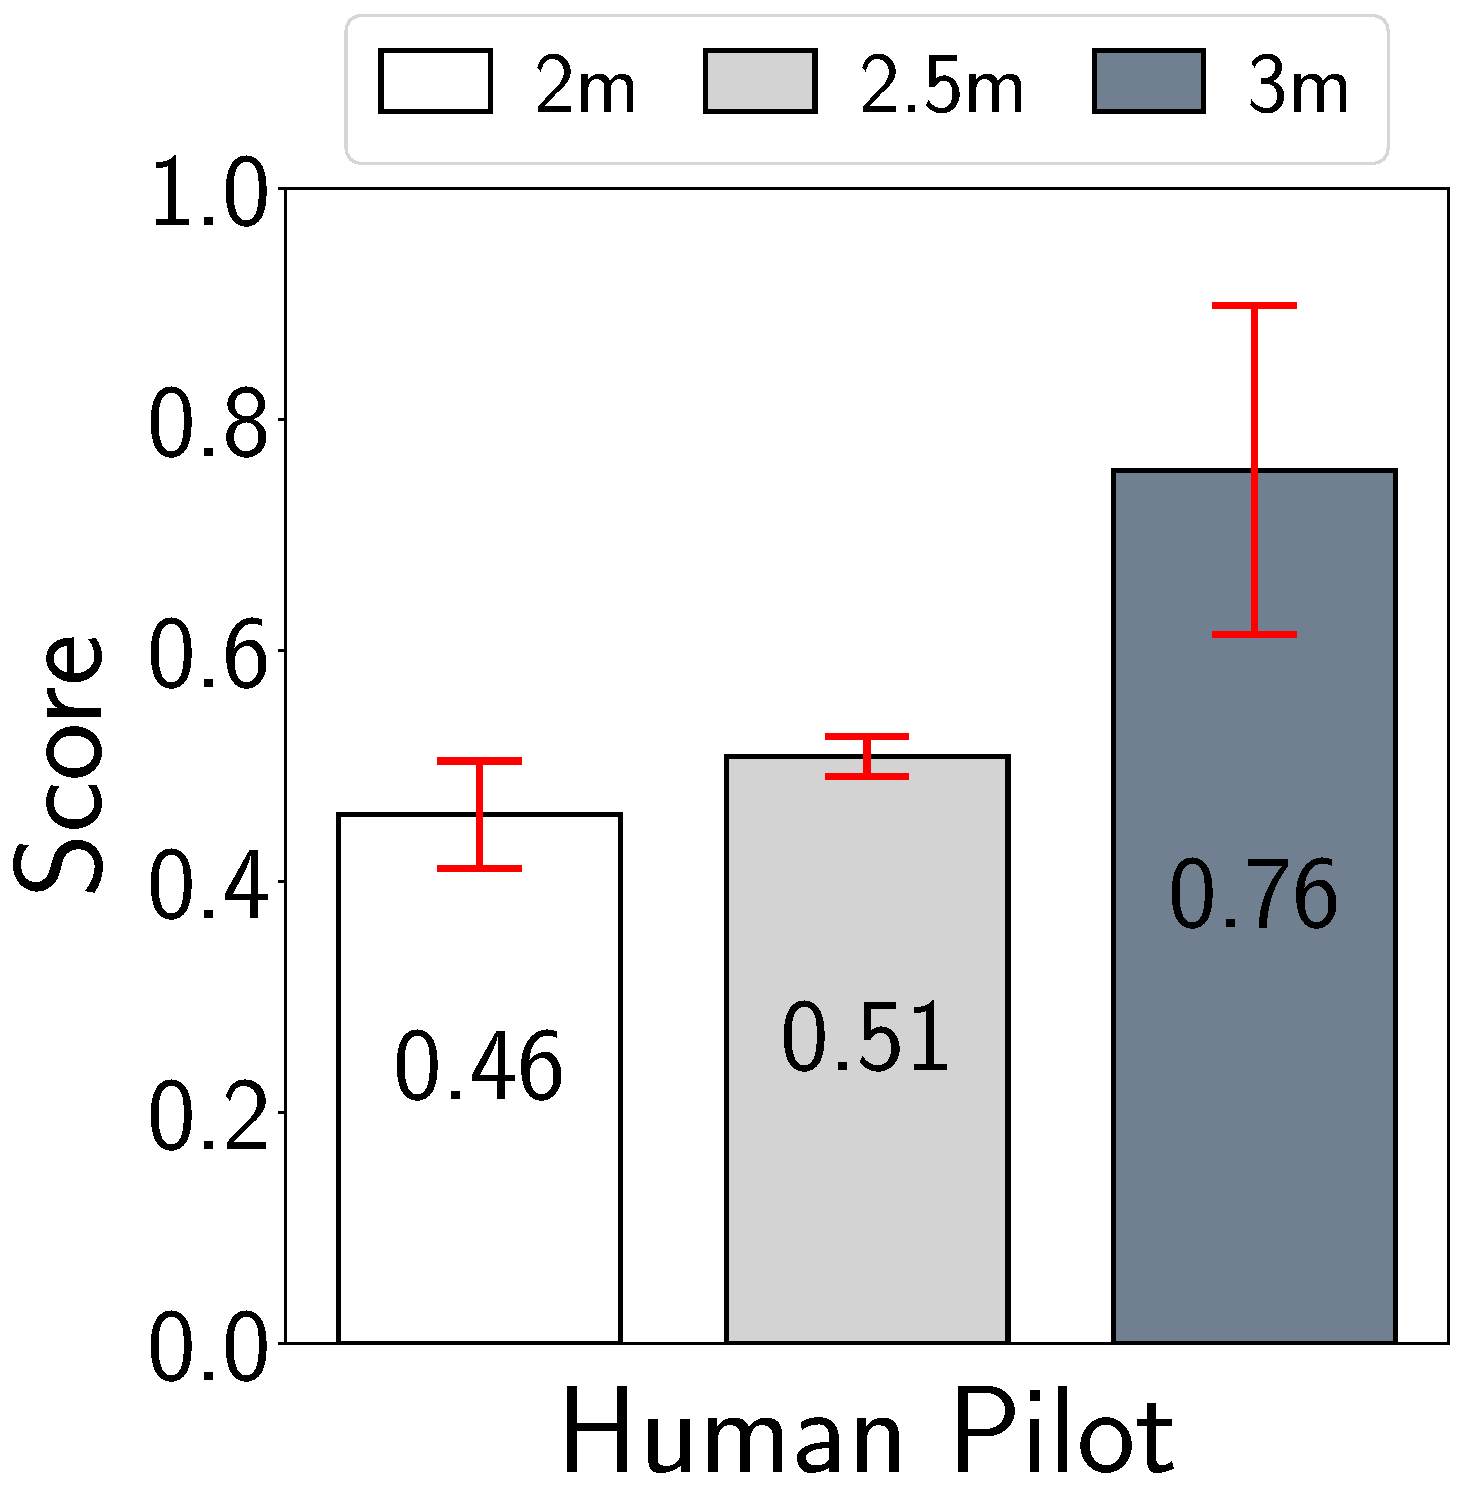
\includegraphics[width=1.0\linewidth]{chapter6/FIGS/fig-avoidance-human.pdf}\\
\caption{Human Pilot}
\label{fig:avoid-human}
\end{minipage}
\end{figure}


\begin{figure}
\centering
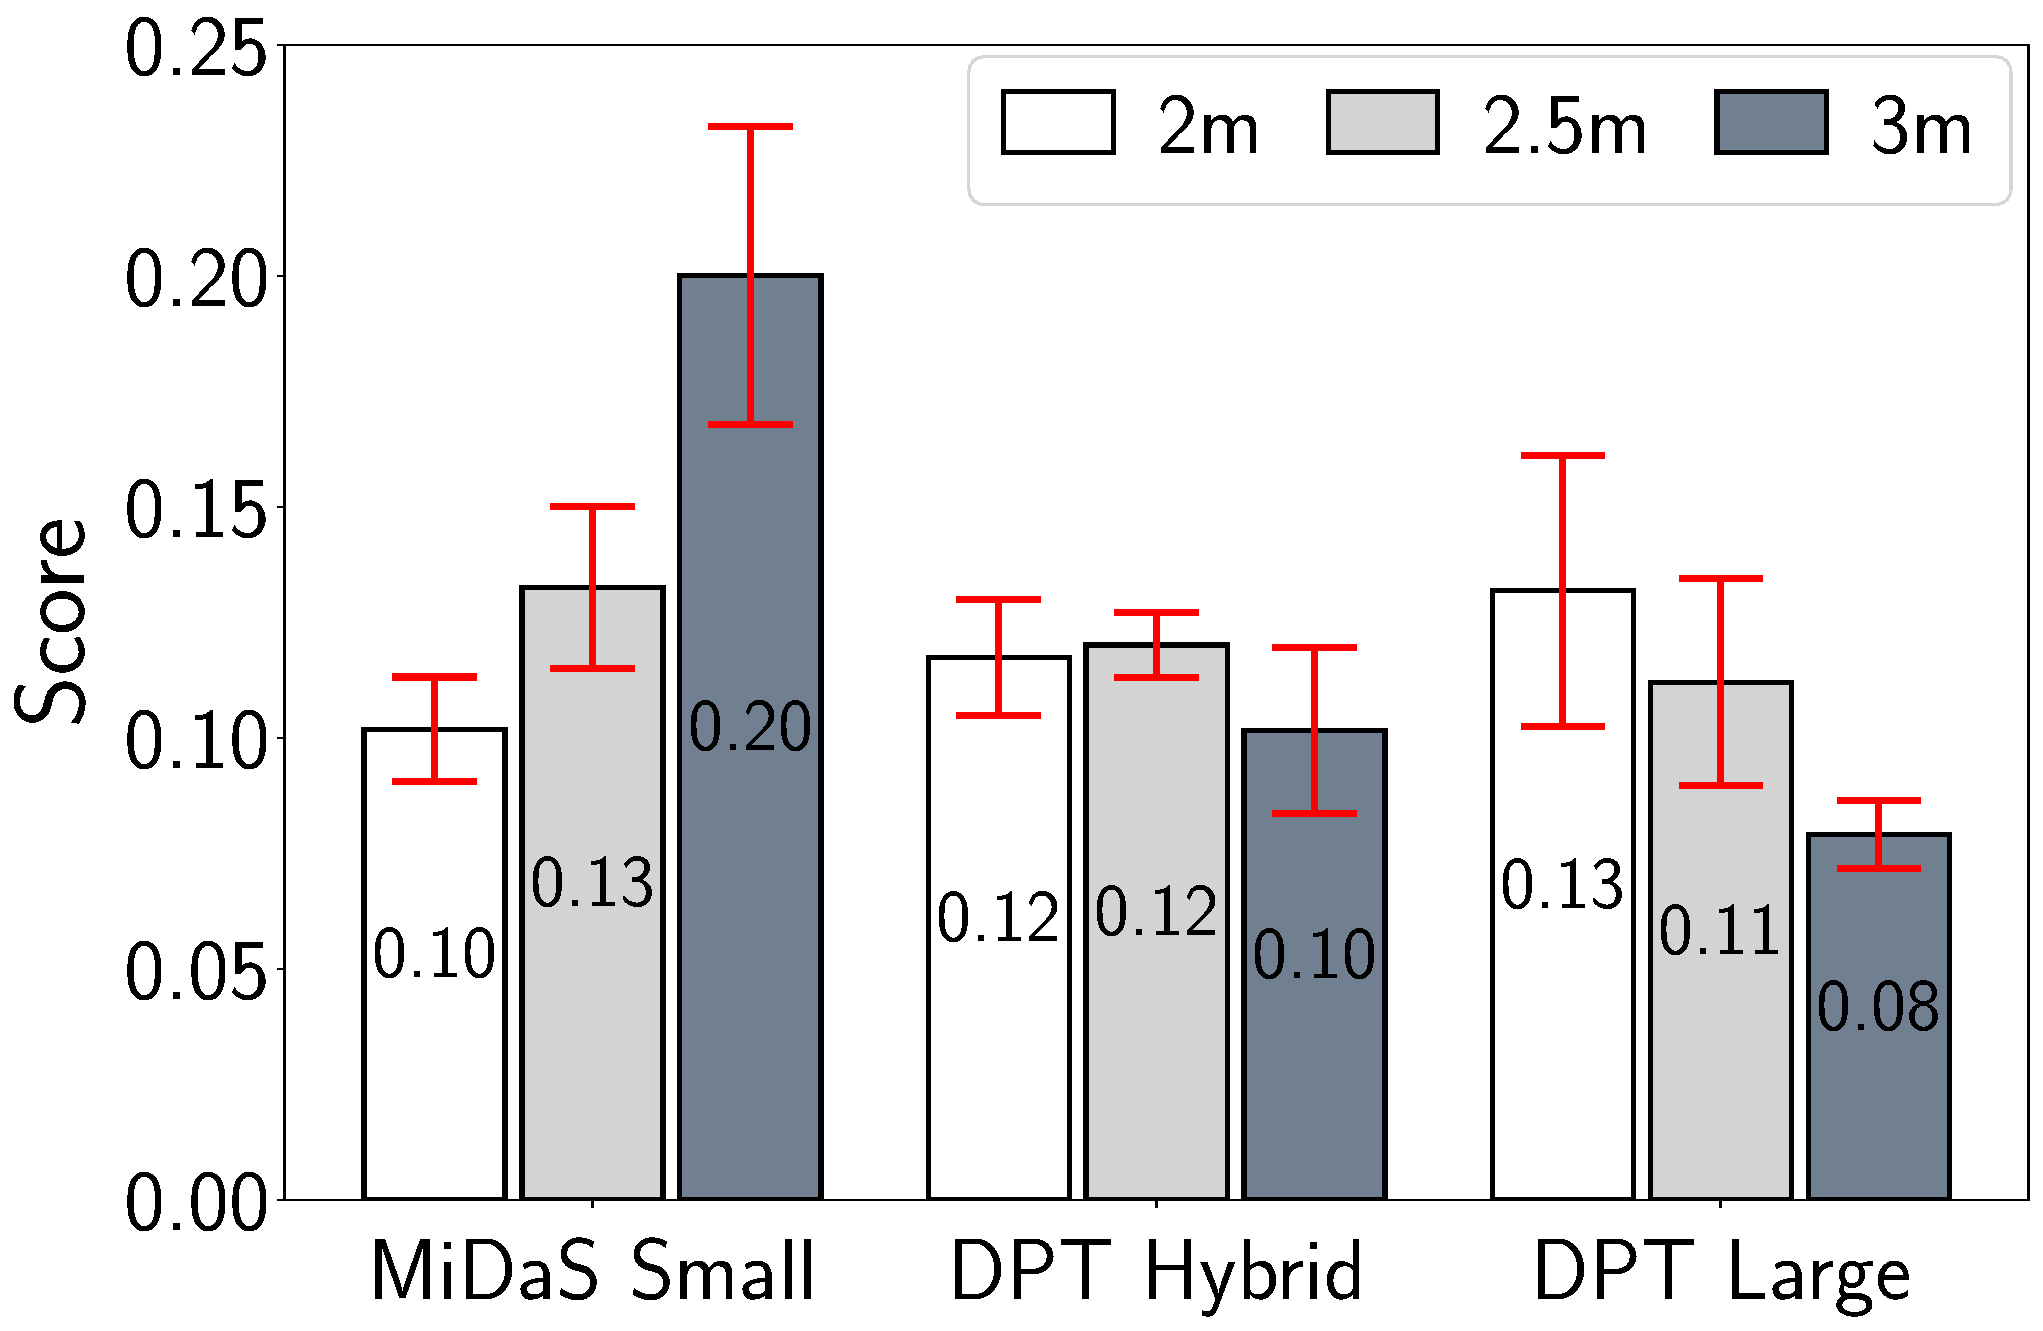
\includegraphics[width=0.8\linewidth]{chapter6/FIGS/fig-avoidance-models.pdf}
\caption{Impact of MiDaS Model on Avoidance Benchmark}
\label{fig:avoidance_by_model}
\end{figure}


\subsection{Impact of Model Accuracy}
\label{sec:avoidance-models}
The availability of the different MiDaS models shown in
Table~\ref{tab:midas-model-stats} leads to the question:
\begin{itemize}
\item{\em Is accuracy or speed  more important?}
\end{itemize}
My experiments indicate that there is no simple answer to this
question.  The results in Figure~\ref{fig:avoid-best} were
obtained using the best MiDaS model for each value of $w$.  MiDaS
Small performs the best on the 3~m course but worst on the 2~m course.
DPT Large is the inverse, performing best on the 2~m course and worst
on the 3~m course.  DPT Hybrid stays consistently in the middle for
all three courses.  The fact that different models had to be used in
each case to obtain the best results indicates that there is no single
``best'' model.  

I conducted a set of experiments to better understand this tradeoff
space.  The results in Figure~\ref{fig:avoidance_by_model} show the
score achieved on the benchmark for each model and value of $w$.
Since MiDaS Small focuses on throughput and low latency over accuracy,
a drone that uses it is able to sustain a higher maximum speed than
one using DPT Large.  At $w = $3~m, the course is sufficiently easy
that the increased risk of collision is small.  The higher accuracy of
a better model is not useful.  However, at $w = $2~m, the increased
likelihood of collisions makes higher model accuracy worthwhile.  Now,
DPT Large attains the highest score.  For a tight course, it is
difficult to travel at high speed without collisions. Hence, a model
that can navigate the gaps better gets a higher  score.

\begin{figure}
\centering
\begin{minipage}{0.8\linewidth}
\centering
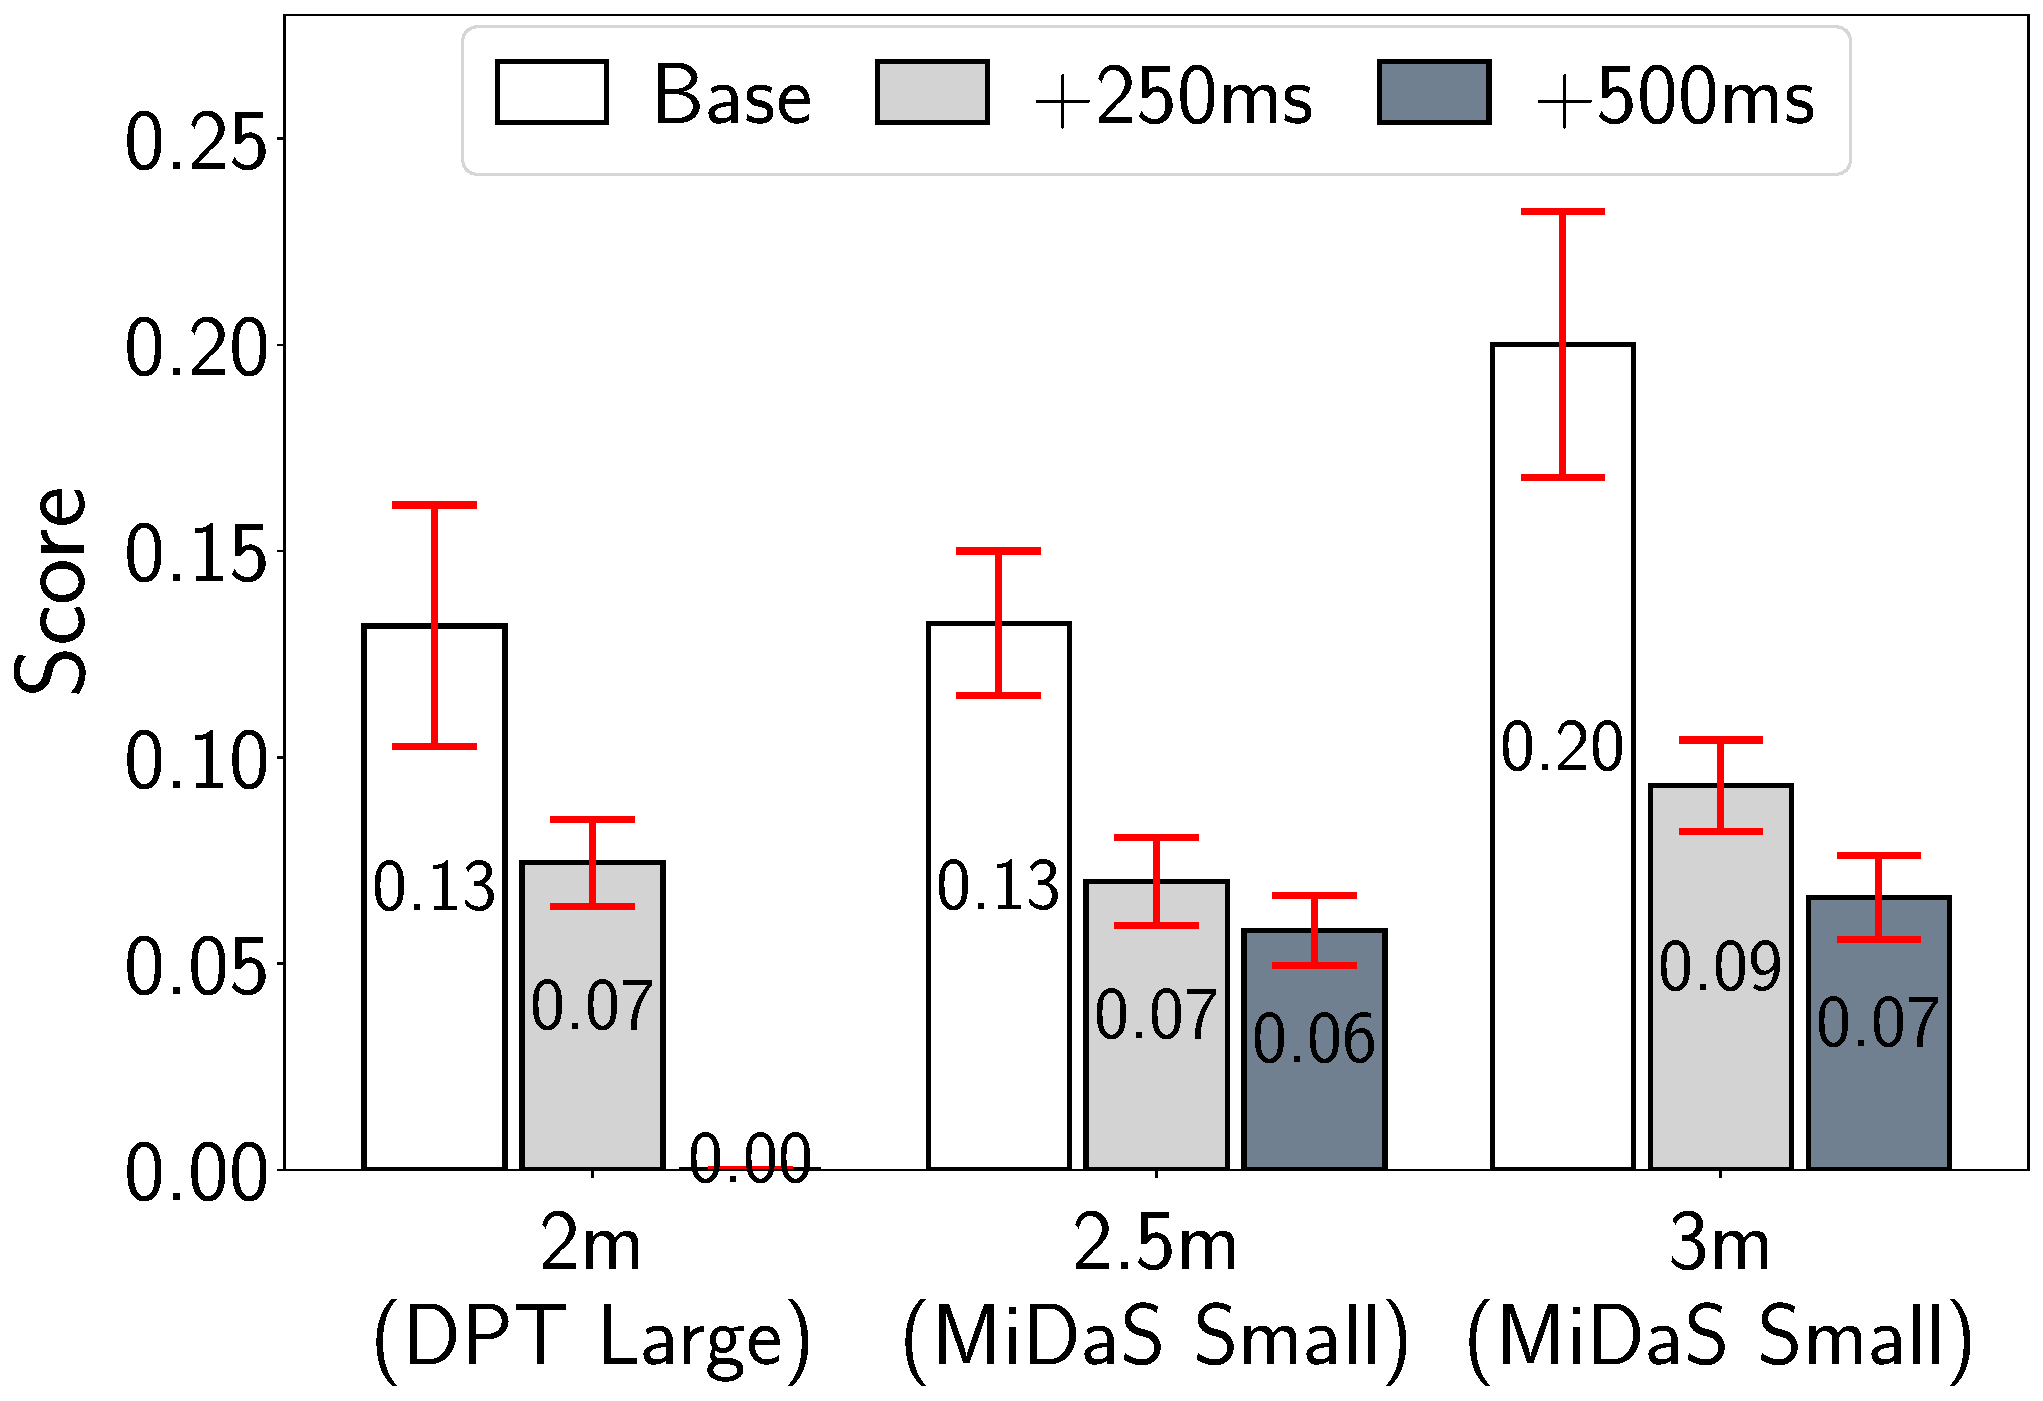
\includegraphics[width=0.96\linewidth]{chapter6/FIGS/fig-avoidance-latency.pdf}
(a) Additional Latency
\end{minipage}
\begin{minipage}{0.8\linewidth}
\centering
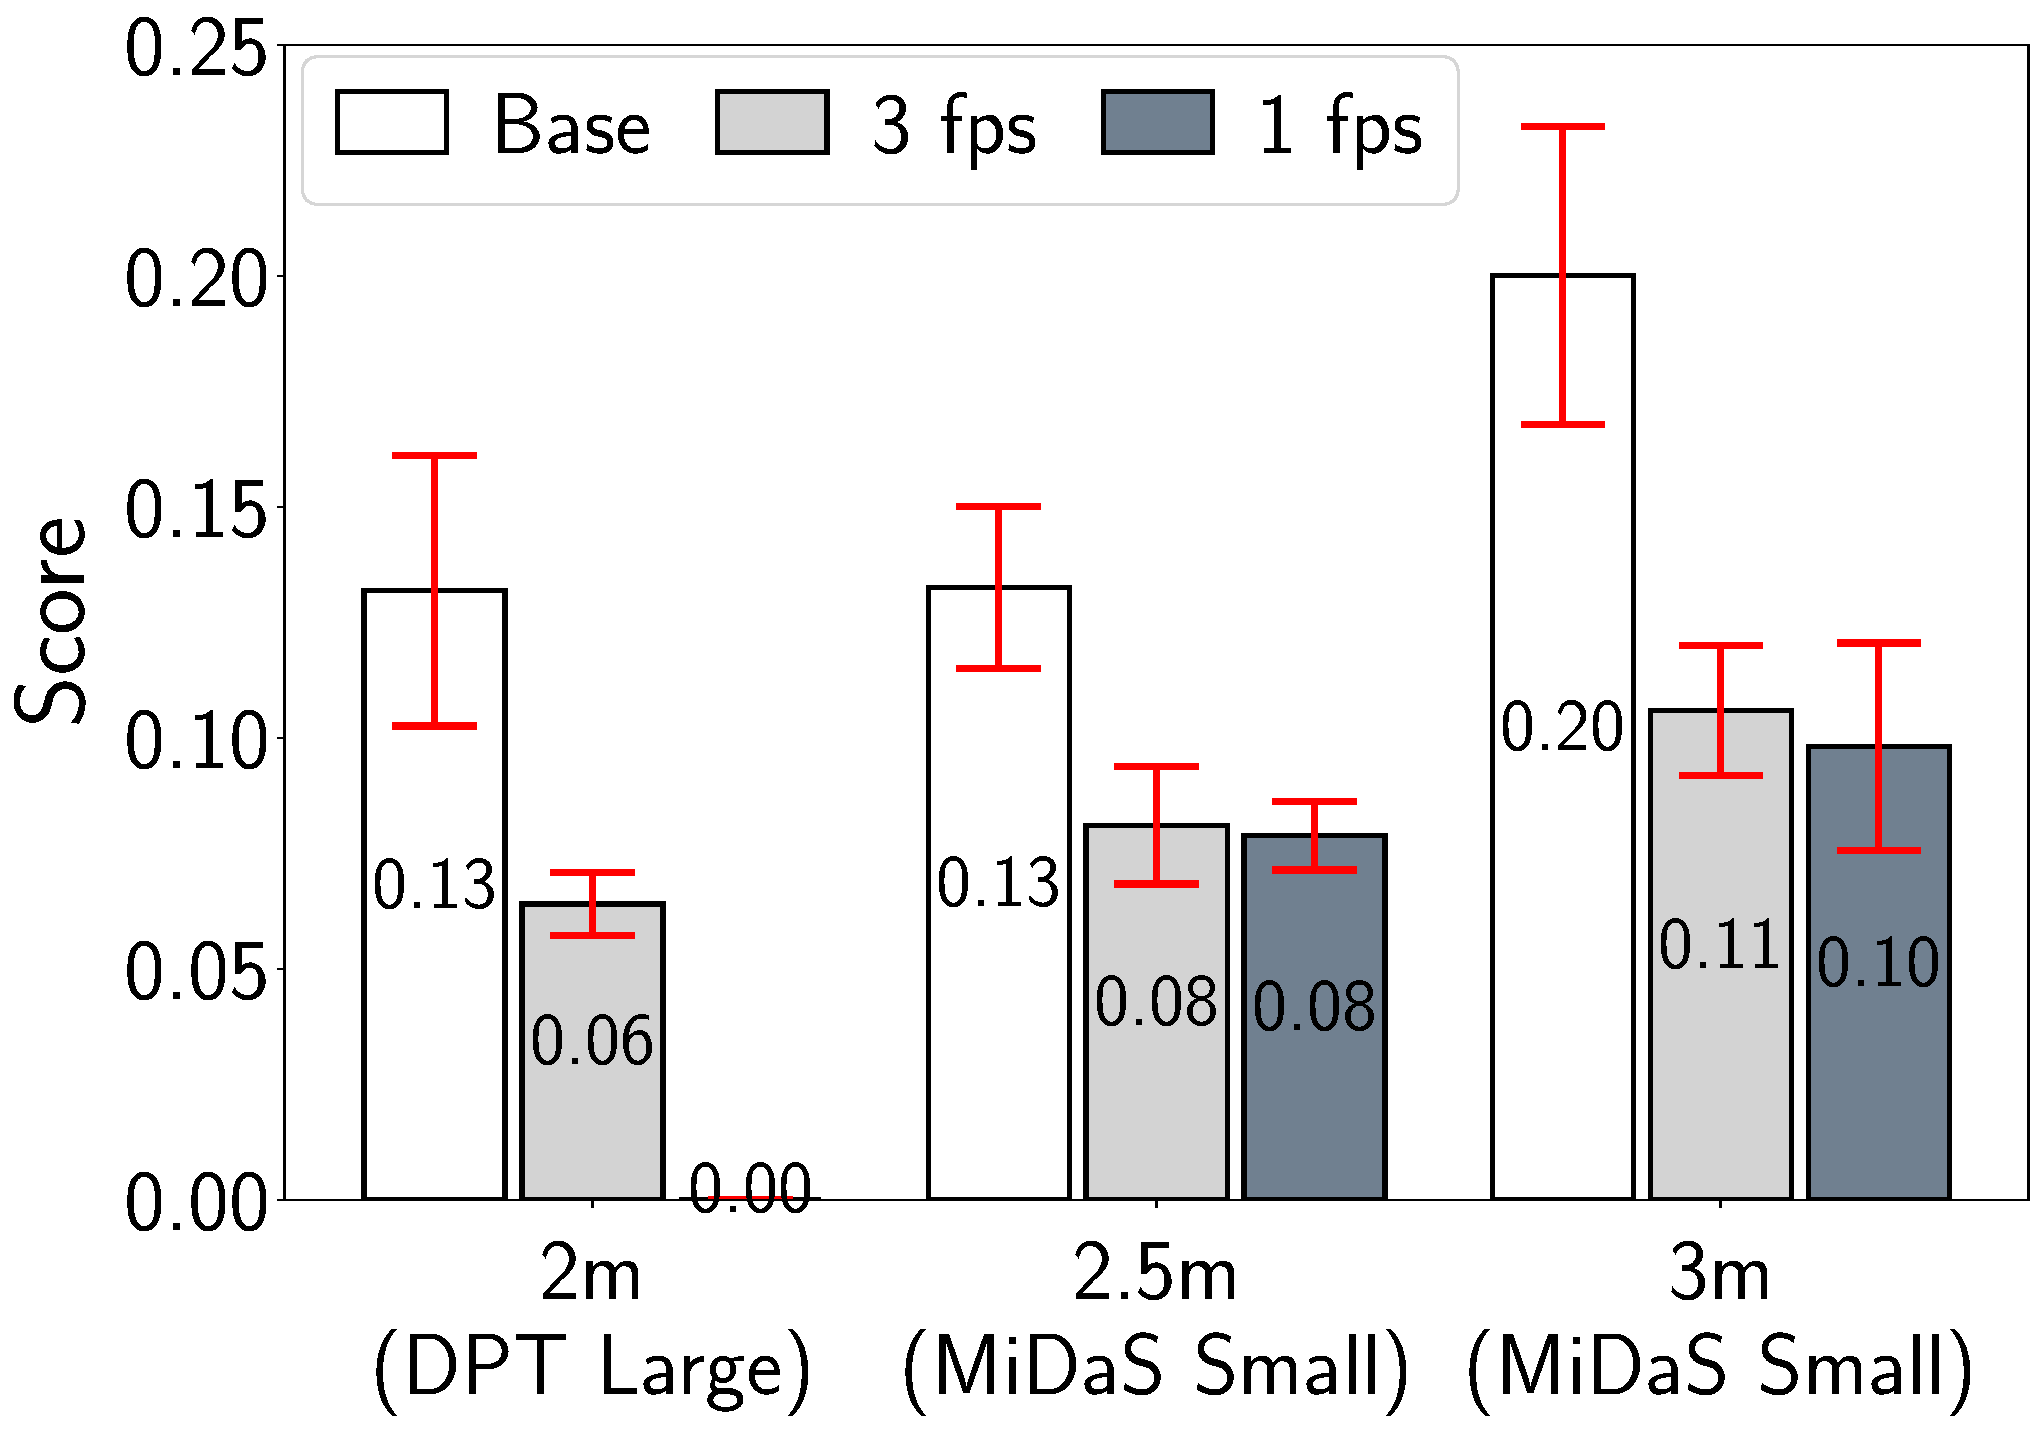
\includegraphics[width=0.96\linewidth]{chapter6/FIGS/fig-avoidance-fps.pdf}
(b) Reduced Throughput
\end{minipage}
\caption{Impact of Latency and Throughput on Avoidance}
\label{fig:avoidance-latency-throughput}
\end{figure}

\subsection{Impact of Latency \& Throughput}
\label{sec:avoidance-factors}

The results presented so far reflect best-case conditions.  In
practice, the wireless network or the cloudlet may suffer degradation
due to multi-tenancy.  This leads to the question:
\begin{itemize}
\item{\em What is the impact of latency or throughput degradation of
    the \ooda~loop on benchmark score?}
\end{itemize}
The baseline scores reflect what is
achievable with an \ooda~loop whose latency is the sum of three
components:
\begin{itemize}
\item{a lower bound of 527~ms~(Figure~\ref{fig:ooda-scaling}).}

\item{the latency of the relevant MiDaS model~(Table~\ref{tab:midas-model-stats}).}

\item{a small additional overhead ($<$1~ms) for Stage-3 processing
    in the Decide part of the \ooda~loop.}
\end{itemize}

This total end-to-end latency is on the order of 600--650~ms.  For
\ooda~loop iterations that involve drone actuation, the bottleneck
throughput is the smaller of 6~fps for
Act$_{fg}$~(\S\ref{sec:c2d-drone}) and the throughput of the MiDaS
model~(Table~\ref{tab:midas-model-stats}).  This is effectively
6~fps, regardless of model.  If no drone actuation is involved, the
bottleneck throughput becomes that of the MiDaS model.  Since even
MiDaS Small has lower throughput than Observe$_{ab}$, Observe$_{c}$,
or best-case Orient+Decide$_d$, throughput is always in the 6--10~fps
range.

Figure~\ref{fig:avoidance-latency-throughput}(a) shows how benchmark
score drops as latency is artificially added to the \ooda \\ loop.  Even
250~ms of additional latency (i.e., a roughly 35--40\% increase from
baseline) causes benchmark score to drop to nearly half its baseline
value, for all values of $w$ and regardless of MiDaS model.  If 500~ms
of latency is added, the score drops further.  For the most
challenging course~($w = 2$~m), the score drops to zero because not
even 80\% of the flights are successful.  These results are consistent
with a long-standing design principle of deeply-immersive closed-loop
interactive systems: {\em increased latency is deadly, even if
  throughput remains good.}

Figure~\ref{fig:avoidance-latency-throughput}(b) shows how benchmark
score drops as the throughput of the \ooda~loop is artificially
reduced from its baseline value.  Reducing throughput to 3~fps causes
benchmark score to drop to nearly 40--50\% of its baseline value.  A
further drop is observed when throughput is reduced to 1~fps.  For $w
= 2$~m, the benchmark score drops to zero.  These results confirm that
latency is not the sole determinant of task performance in an
\ooda~loop --- throughput also matters.

\subsection{Value of On-board Drone Intelligence}
\label{sec:djiminipro}

Edge computing allows use of compute resources that are far larger and heavier than could be carried by an ultralight drone.  In the context of AI,
this translates to {\em generality} and {\em versatility}.  Purely
through software development on the cloudlet, it is easy to re-purpose
the drone for new tasks that were not anticipated earlier.

\begin{figure}
\small
\centering
\begin{tabular}{lr}
  \hline
  Architecture & Efficiency (GFLOP / J) \\
  \hline
  CPU (Core i7)        & \phantom{0}1.14  \\
  FPGA (Xilinx LX760)  & \phantom{0}3.62  \\
  GPU (NVIDIA GTX285)  & \phantom{0}6.78  \\
  GPU (AMD R5870)      & \phantom{0}9.87  \\
  ASIC                 & 50.73 \\
  \hline
\end{tabular}
\begin{captext}
\\[0.2cm] \small Source: Table 4 in Chung et al~\cite{Chung2010}
\end{captext}
\caption{Matrix Multiplication Kernel Implementations}
\label{fig:energy2}
\end{figure}

The drone marketplace, however, is moving in the opposite direction.
Drone vendors are constantly identifying specific new functionality to
add to drones. There is a well-understood tradeoff between
generality, energy-efficiency, development cost, and weight/size that
applies in this context. As Figure~\ref{fig:energy2} from Chung et
al~\cite{Chung2010} shows, an ASIC is by far the most energy efficient
alternative for a given functionality.  It is also likely to have the
lowest weight.  But, it takes much longer to develop, is much more
expensive to create than pure software, and only provides fixed
functionality.

To quantify the value of on-board intelligence, I re-ran my obstacle
avoidance benchmark using a DJI Mini 4 Pro drone, seen in Figure~\ref{fig:drone-anatomy}.  This consumer
photography drone weighs 249~g, and is equipped with 6 stereo cameras
and an onboard obstacle avoidance system. It has two modes, Normal and
Nifty. Normal prioritizes safe flight while Nifty attempts to pass
obstacles as quickly as possible.  The obstacle avoidance feature of
this drone is intended as a form of ``pilot assist.''  The RPIC flies
the drone without worrying about obstacles.  The drone's builtin
capability performs all the necessary sensing and actuation needed to
avoid collisions.

Figure~\ref{fig:avoidance_dji} presents the scores obtained by the DJI
Mini 4 Pro  on my obstacle avoidance benchmark.  The baseline results
for my platform from Figure~\ref{fig:avoid-best} are also shown for
comparison.  For all values of $w$, the DJI Mini 4 Pro  is at a clear
advantage.  This the direct result of additional sensors and a much
faster \ooda~loop that avoids edge offload.

\begin{figure}
\centering
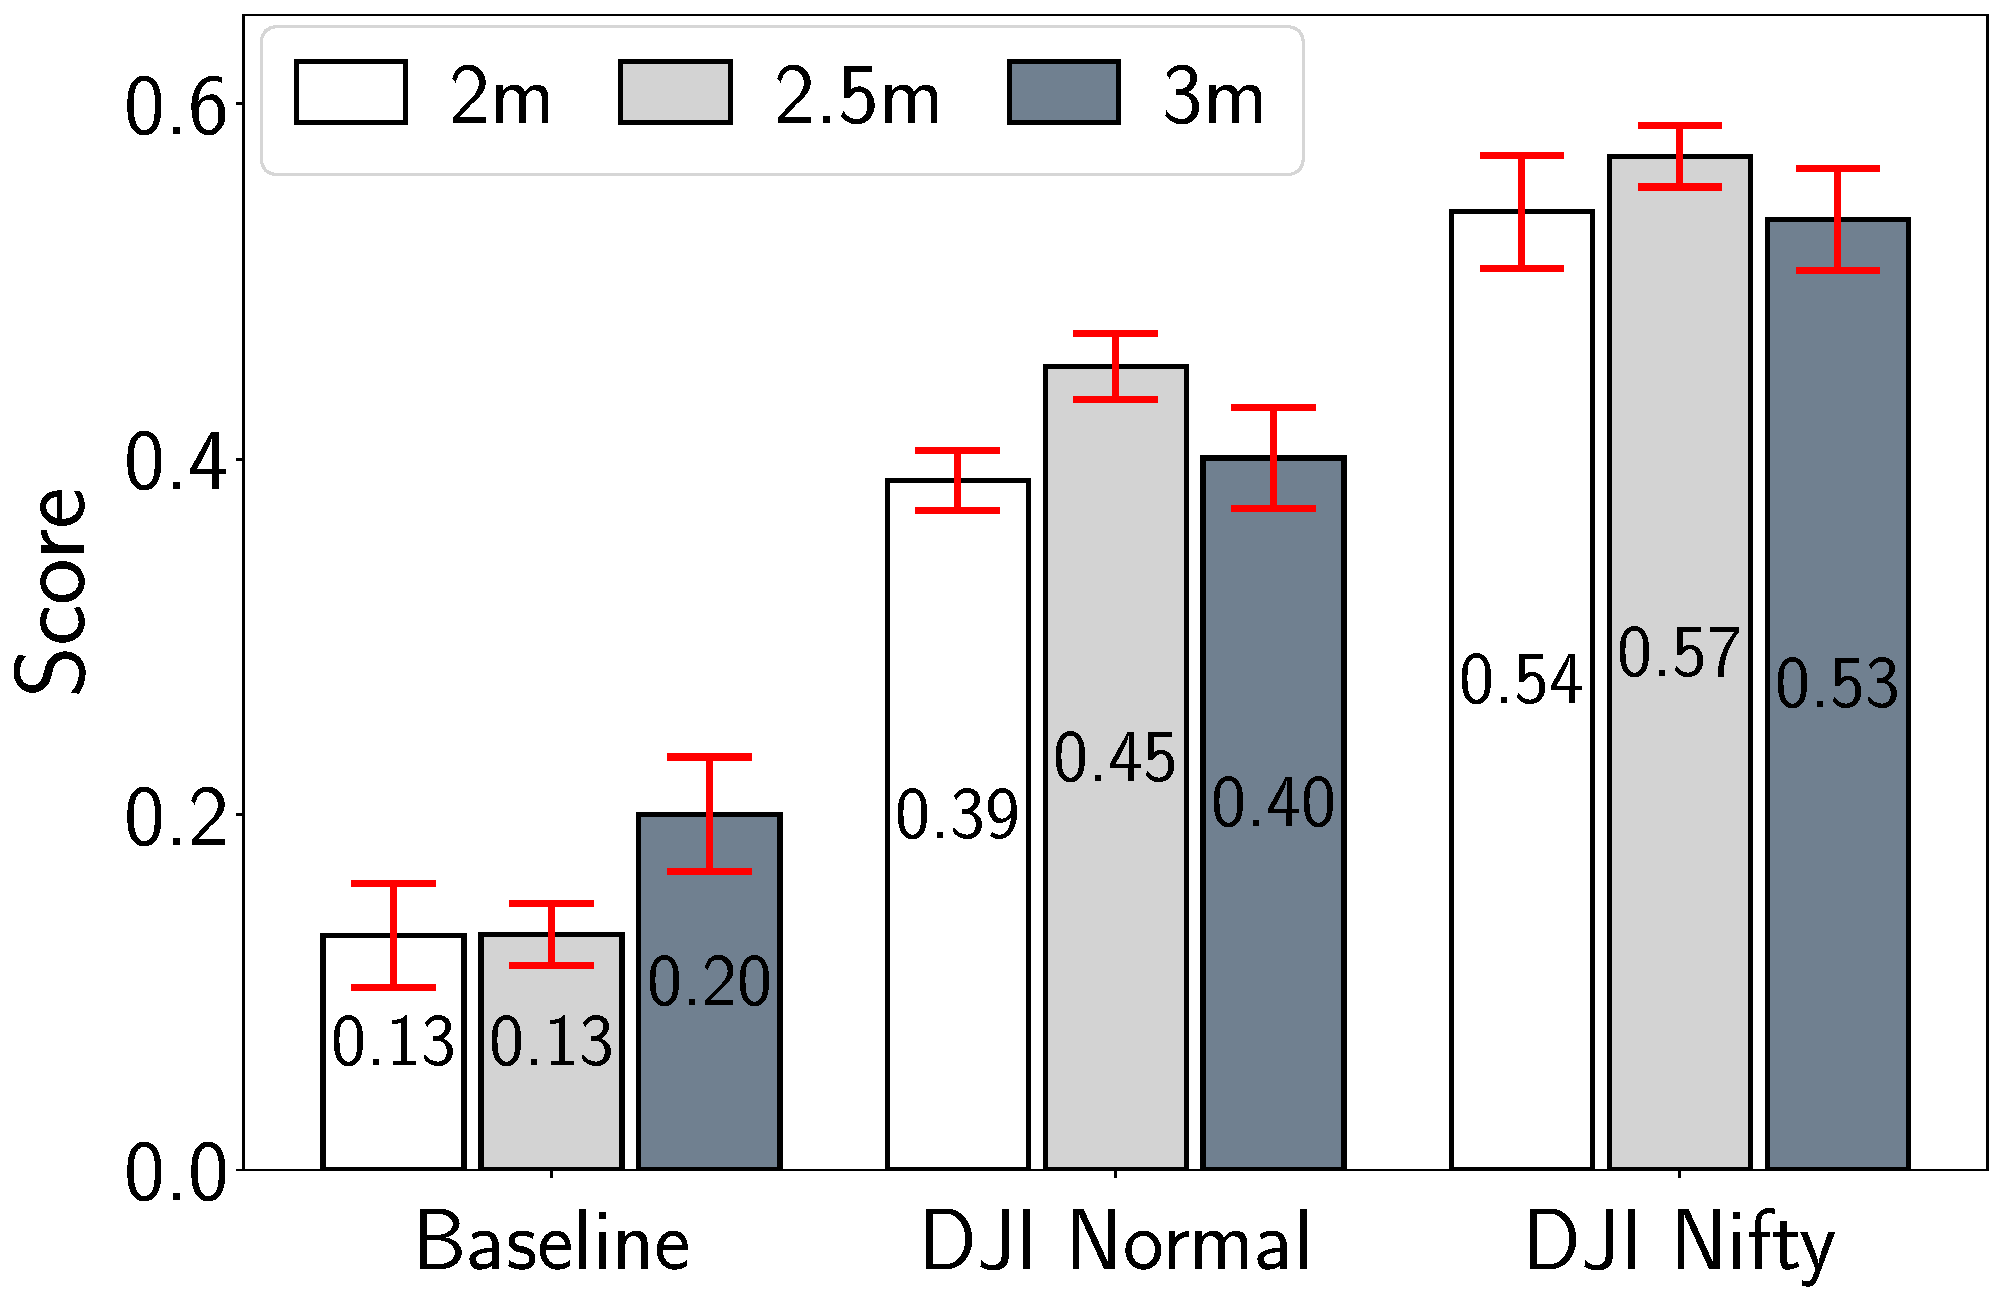
\includegraphics[width=0.8\linewidth]{chapter6/FIGS/fig-avoidance-dji.pdf}
\caption{On-Board Obstacle Avoidance}
\label{fig:avoidance_dji}
\end{figure}

These results suggest that even when using edge offload, there is very
clear value in taking advantage of on-board capabilities when they are
available.  The ``pilot assist'' approach to obstacle avoidance
implemented by the DJI Mini 4 Pro could equally well be used by
cloudlet-based software to control the drone's flight path.  Only the
macro components of that flight path would incur the overhead of the
\ooda~loop from drone to cloudlet.  The micro components of the flight
path that maneuver the drone around obstacles would only be subject to
its much tighter on-board \ooda~loop.

Complementing on-board fixed functionality with edge offload provides
extensibility and versatility.  The DJI Mini 4 Pro, for example, is
unable to do general-purpose object detection even though it can
detect people and vehicles.  It cannot detect the Robomaster target, and is hence
unable to execute my tracking benchmark.  Edge offload could remedy
that limitation, thereby increasing the versatility of the drone.




